\chapter{Lưu trữ dữ liệu}
\label{chap:chuong1}
\minitoc 
\vspace{0.5cm}
\noindent
Trong chương này, ta sẽ xem xét cách dữ liệu được biểu diễn và lưu trữ trong máy tính.  Cụ
thể, ta sẽ xem xét cách biểu diễn văn bản, giá trị số, âm thanh, hình ảnh và video. Nhiều
thông tin trong chương này cũng thích hợp với các lĩnh vực khác như ảnh số, sản xuất và
thu âm audio/video, và truyền thông khoảng cách xa.

  
\section{Các bít và cách lưu trữ}

Máy tính thực chất là một máy điện, nó hoạt động dựa theo nguyên tắc lựa chọn tắt hoặc mở
hàng triệu chuyển mạch rất nhỏ bên trong nó. Các trạng thái tắt hoặc bật này được mã hoá
dưới dạng các số $0$ hoặc $1$. Các số này được gọi là các bít (gọi tắt của \textit{số nhị
  phân}).


Thông tin trong máy tính được biểu diễn dưới dạng dưới dạng dãy bít~0 hoặc~1, và dù rằng
ta nhìn các bít như giá trị số thì chúng thực sự vẫn chỉ là ký hiệu hình thức, ý nghĩa của
nó tuỳ thuộc từng cách áp dụng--lúc chúng được dùng để biển diễn giá trị số, lúc chúng
được dùng để biểu diễn ký tự trên một bảng chữ nào đó, lúc này chúng là biểu diễn hình
ảnh, lúc khác lại là biểu diễn âm thanh.

\subsection*{Phép toán Boolean}

Nếu ta xem bít $0$ biểu diễn một giá trị logic \textit{false} và bít $1$ biểu diễn cho giá
trị \textit{true} thì các thao tác bên trong máy tính có thể được mô tả một cách hình thức
bởi các \textbf{phép toán Boolean}, theo tên của George~Boole (1815-1864), một người đi
tiên phong trong Logic toán. Hình  \ref{fig:op-bool1} liệt kê ba trong nhiều phép toán
boolean: AND, OR, XOR. Các phép toán này về mặt hình thức tương tự như các phép toán hai
ngôi Nhân, Cộng và Trừ trong số học, chúng cũng nhận hai tham số đầu vào và trả ra kết
quả. Ví dụ, phép toán AND với đầu vào là cặp giá trị false~($0$) và true~($1$) sẽ cho kết
quả là false~($0$); cụ thể ta có:
\[
  0 \AND 1 = 0.
\] 
Khác ba phép toán đề cập ở trên, phép toán $\NOT$ là phép toán một ngôi, nó chỉ có một đầu
vào và một đầu ra. Trong đó đầu ra là giá trị đảo của đầu vào:
\[
\NOT  0 = 1 \mbox{ và } \NOT 1 = 0.
\]

\begin{figure}[tb]
\centering
  \begin{minipage}{1.5in}
    \begin{tabular}{cc|c}
      $p$ & $q$ & $p \AND q$ \\
      \hline
      0 & 0 & 0 \\
      0 & 1 & 0 \\
      1 & 0 & 0 \\
      1 & 1 & 1
    \end{tabular}
  \end{minipage}
  \begin{minipage}{1.5in}
    \begin{tabular}{cc|c}
      $p$ & $q$ & $p \OR q$ \\
      \hline
      0 & 0 & 0 \\
      0 & 1 & 1 \\
      1 & 0 & 1 \\
      1 & 1 & 1
    \end{tabular}
  \end{minipage}
  \begin{minipage}{1.5in}
    \begin{tabular}{cc|c}
      $p$ & $q$ & $p \XOR q$ \\
      \hline
      0 & 0 & 0 \\
      0 & 1 & 1 \\
      1 & 0 & 1 \\
      1 & 1 & 0
    \end{tabular}
  \end{minipage}
  \caption{Các phép toán AND, OR, XOR (tuyển loại). Hai cột đầu tiên biểu diễn tham số đầu
    vào, cột thứ ba chỉ kết quả của phép toán tương ứng với tham số đó.}
    \label{fig:op-bool1}
\end{figure}

\subsection*{Các cổng logic và Flip-Flop} 

%Các kết quả của đại số Boolean rất quan trọng trong thiết kế các thành phần của máy tính. Ý tưởng cơ bản là xây dựng các mạch đơn giản thực hiện một vài phép toán Boolean, còn các mạch phức tạp hơn có thể xây dựng lại được bằng cách kết hợp các mạch đơn giản đó.

\begin{figure}[tbh]  
\centering

\subfloat[Cổng logic $\AND$]{
  \begin{minipage}{3in}
\begin{center}
    \scalebox{0.5}{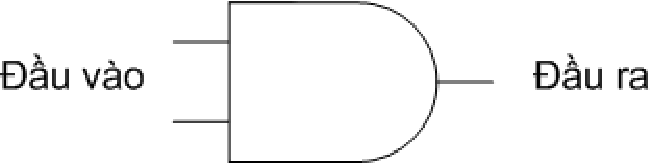
\includegraphics{ch2/fig2and.pdf}}

    \vspace{0.5cm}
    \begin{tabular}{cc|c}
      \multicolumn{2}{c|}{Đầu vào} &  Đầu ra \\
      \hline
      0 & 0 & 0 \\
      0 & 1 & 0 \\
      1 & 0 & 0 \\
      1 & 1 & 1
    \end{tabular}
  \end{center}
\end{minipage}
}
\subfloat[Cổng logic $\OR$]{
  \begin{minipage}{3in}
    \begin{center}
      \scalebox{0.5}{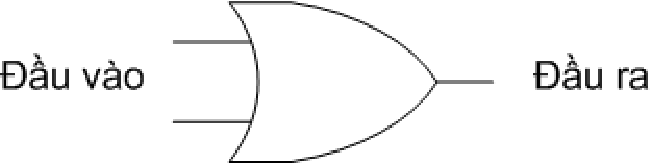
\includegraphics{ch2/fig2or.pdf}} 

      \vspace{0.5cm}
      \begin{tabular}{cc|c}
      \multicolumn{2}{c|}{Đầu vào} &  Đầu ra \\
      \hline
      0 & 0 & 0 \\
      0 & 1 & 1 \\
      1 & 0 & 1 \\
      1 & 1 & 1
    \end{tabular}
  \end{center}
\end{minipage}
}

\vspace{0.7cm}

\subfloat[Cổng logic $\XOR$]{
  \begin{minipage}{3in}
    \begin{center}
      \scalebox{0.5}{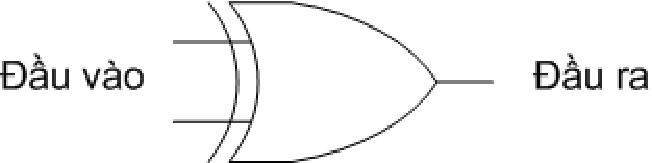
\includegraphics{ch2/fig2xor.pdf}}

      \vspace{0.5cm}
      \begin{tabular}{cc|c}
        \multicolumn{2}{c|}{Đầu vào} &  Đầu ra \\
        \hline
        0 & 0 & 0 \\
        0 & 1 & 1 \\
        1 & 0 & 1 \\
        1 & 1 & 0
      \end{tabular}
    \end{center}
\end{minipage}
}
\subfloat[Cổng logic $\NOT$]{
  \begin{minipage}{3in}
    \begin{center}
      \scalebox{0.5}{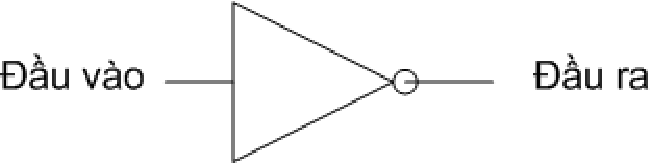
\includegraphics{ch2/fig2not.pdf}} 

\vspace{0.5cm}
      \begin{tabular}{c|c}
        Đầu vào &  Đầu ra \\
        \hline
        0 & 0 \\
        1  & 0 
      \end{tabular}
    \end{center}
  \end{minipage}
} 

\vspace{0.3cm}
\caption{Các cổng logic}
\label{fig:op-bool2}
\end{figure}


\begin{figure}[tbh]  
\centering
    \scalebox{0.4}{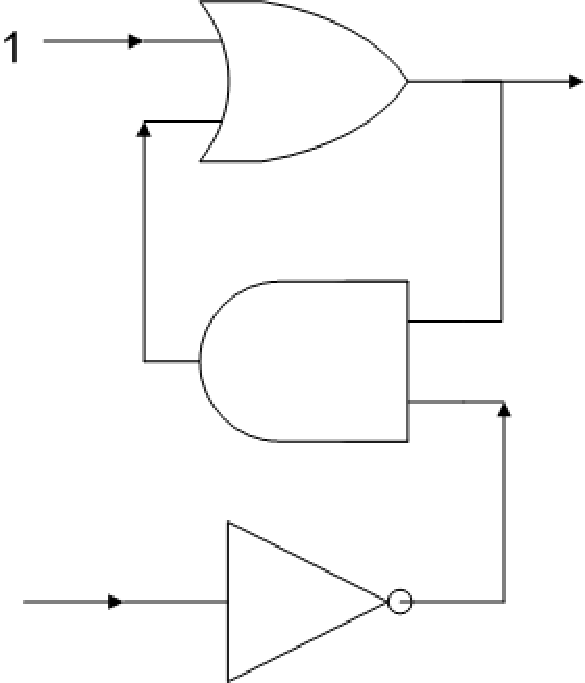
\includegraphics{ch2/fig-fflp.pdf}}
\caption{Một mạch Flip-Flop}
 \label{fig:op-flipflop}
\end{figure}
 

\textbf{Cổng} là một thiết bị điện tử có một hoặc nhiều đầu vào, mỗi đầu vào nhận giá trị
$0$ hoặc~$1$, tương ứng với hai mức điện thế; và thường có một đầu ra, đó là một hàm theo
đầu vào, nó cũng nhận giá trị~$0$ hoặc~$1$.  Trong giáo trình này, ta sẽ chỉ xem xét một
cách hình thức các cổng như các ký hiệu, bỏ qua cách biểu diễn vật lý của chúng.

Một cổng thường để tính toán một hàm Boolean cụ thể, đơn giản nào đó. Trong nghành công
nghiệp điện tử, người ta thường chỉ xây dựng một số cổng thực hiện một vài hàm nhất định,
còn các hàm khác sẽ được xây dựng lại bằng cách tổ hợp các cổng cơ bản đó.  Một số cổng
quen thuộc được liệt kê trong Hình~\ref{fig:op-bool2}.

 
Các cổng được tổ hợp thành các \textbf{mạch số} (gọi tắt là mạch) bằng cách nối đầu ra của
một số cổng với đầu vào một số cổng khác. Mỗi mạch có thể có một hoặc nhiều đầu vào, mỗi
đầu vào này lại có thể là đầu vào của nhiều cổng khác bên trong mạch. Đầu ra của mạch là đầu ra của một hoặc
nhiều cổng trong mạch.

Một mạch quan trọng trong thiết kế các phần tử nhớ được chỉ ra trong Hình~\ref{fig:op-flipflop}, nó được gọi là mạch Flip-Flop. Một Flip-Flop là một mạch được thiết
kế để giữ giá trị đầu ra ($0$ hoặc~$1$) không thay đổi cho tới khi nhận được tín hiệu từ
đầu vào yêu cầu chuyển sang một giá trị khác. Để ý rằng, khác với các phép toán Boolean
trước, giá trị đầu ra của mạch kiểu này không chỉ phụ thuộc đầu vào ở thời điểm hiện tại
mà còn phụ thuộc cả vào đầu ra của thời điểm trước nữa.

Ta khẳng định rằng: khi cả hai giá trị đầu vào của mạch trong Hình \ref{fig:op-flipflop}
đều là~$0$ thì đầu ra của mạch không thay đổi (dù nó có là $0$ hay $1$). Tuy nhiên, khi ta
đặt giá trị $1$ cho đầu vào phía trên của mạch, ngay lập tức đầu ra sẽ là~$1$. Còn khi ta
đặt giá trị $1$ cho đầu vào phía dưới, ngay lập tức đầu ra của mạch sẽ là $0$.


\begin{figure}[tbh] 
\centering
\subfloat[Đặt $1$ và $0$ vào 2 đầu vào]{
    \scalebox{0.35}{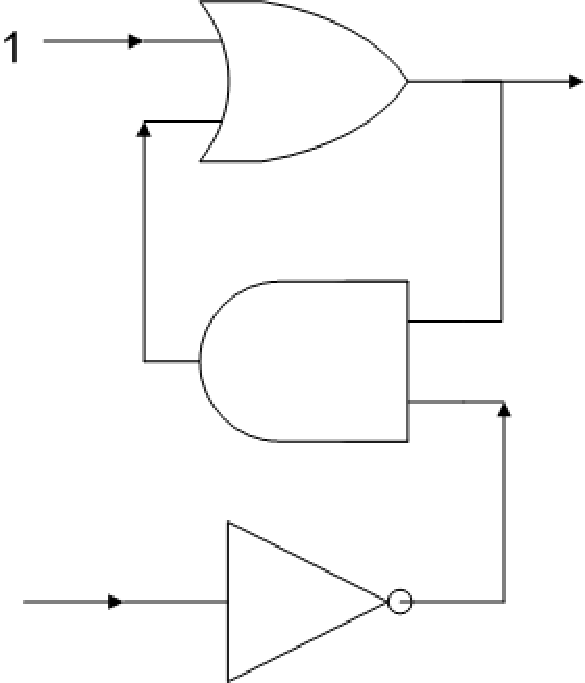
\includegraphics{ch2/figffl1.pdf}}
\label{op-flipflop2a}
}\qquad \subfloat[Đầu ra của cổng $\OR$ và cổng $\AND$ đều là $1$]{
  \scalebox{0.35}{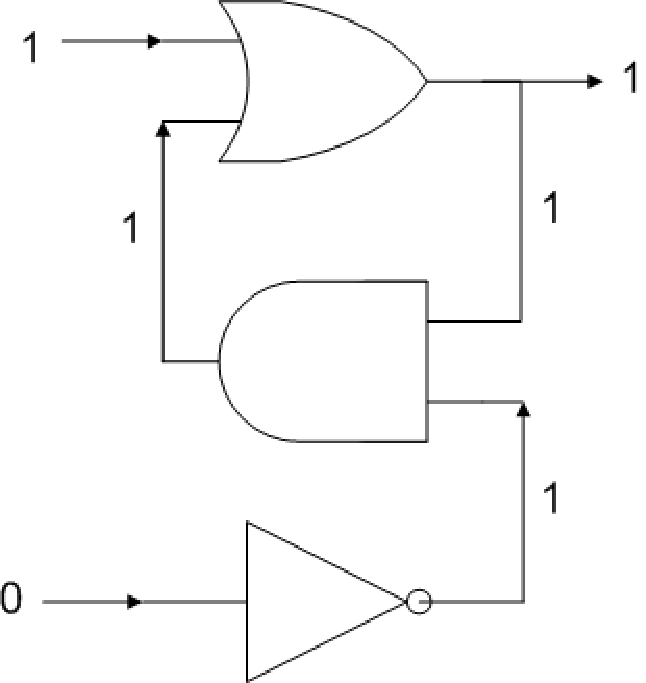
\includegraphics{ch2/figffl2.pdf}}
\label{op-flipflop2b}
} \qquad \subfloat[Giá trị $1$ từ cổng $\AND$ giữ cho đầu ra của $\OR$
bằng $1$ dù đầu vào kia bằng $0$]{
  \scalebox{0.35}{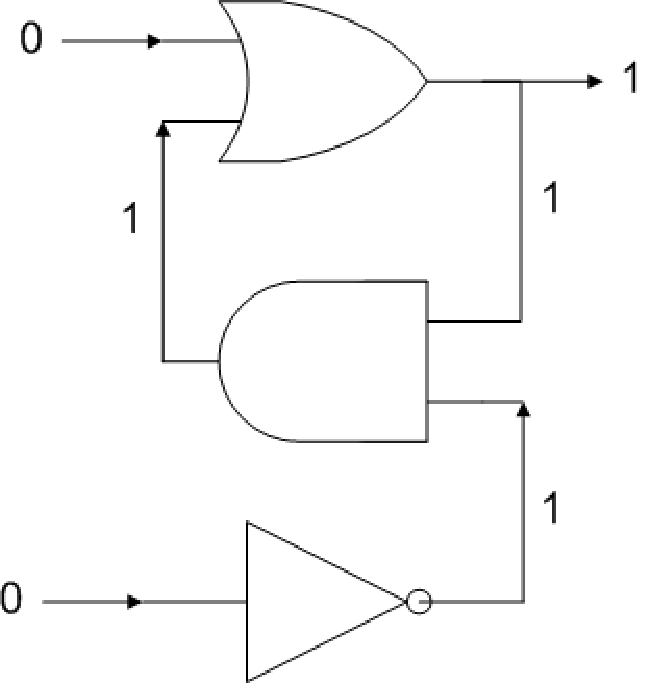
\includegraphics{ch2/figffl3.pdf}}
\label{op-flipflop2c}
}
\caption{Đưa giá trị đầu ra của Flip-Flop lên 1}
\label{fig:op-flipflop2}
\end{figure}

Ta sẽ cùng phân tích khẳng định trên một cách chi tiết. Trước hết, ta thấy rằng dù đầu ra
của mạch~\ref{fig:op-flipflop} là gì đi nữa, nếu đầu vào phía trên của mạch đặt
bằng~$1$ và phía dưới đặt bằng $0$, vậy đầu ra của cổng $\OR$ sẽ là~$1$. Bây giờ, cả hai
đầu vào của cổng $\AND$ đều bằng $1$, vậy đầu ra của nó bằng $1$, có nghĩa rằng đầu vào
thứ hai của $\OR$ sẽ là~$1$ (Hình~\ref{op-flipflop2b}). Điều này làm cho đầu ra của $\OR$
vẫn bằng $1$, kể cả khi bây giờ đầu vào phía trên của mạch được đặt bằng $0$ (Hình~\ref{op-flipflop2c}).  Tóm lại, đầu ra của Flip-Flop đã trở thành $1$ và luôn giữ ở giá
trị đó dù đầu vào phía trên được đặt bằng $0$ hay không.
 

Cũng tương tự như trên, khi đặt giá trị $1$ cho đầu vào phía dưới sẽ làm cho đầu ra của
Flip-Flop là $0$ và giá trị này vẫn giữ nguyên khi giá trị đầu vào được đưa trở về~$0$.
   
Ta trình bày mạch Flip-Flop trong Hình~\ref{fig:op-flipflop} và Hình~\ref{fig:op-flipflop2}
với hai mục đích. Thứ nhất, nó chỉ ra làm thế nào các thiết bị có thể được xây dựng từ
các cổng, quá trình này được gọi là thiết kế mạch số, nó đóng vai trò quan trọng trong
nghành công nghệ máy tính. Thứ hai, nó cho ta cách để lưu trữ một bít trong máy tính. Thật
vậy, mạch Flip-Flop cho phép ta đặt giá trị để đầu ra của nó luôn bằng $0$ hoặc bằng
$1$. Vậy các mạch khác muốn lưu trữ có thể gửi tín hiệu tới đầu vào của Flip-Flop để đặt
giá trị, và các mạch khác nữa có thể sử dụng giá trị lưu trữ bằng cách lấy giá trị từ đầu
ra của Flip-Flop như đầu vào của nó. Với kỹ thuật hiện nay, rất nhiều Flip-Flop có thể
được kết hợp lại trong một chip và được sử dụng để lưu trữ thông tin dưới dạng mã hoá như
dãy bít~$0$ và~$1$.

\subsection*{Bài tập}
\begin{enumerate}
 \item Với những giá trị đầu vào nào thì mạch sau đây cho đầu ra là $1$?
    \begin{center}
      \scalebox{0.55}{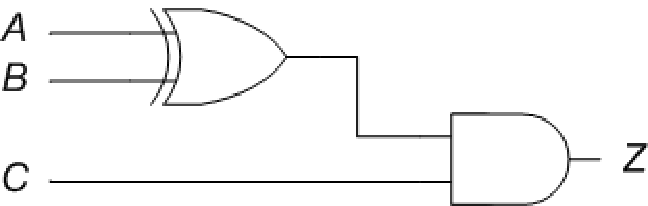
\includegraphics{ch2/bt1.pdf}}
    \end{center}

 \item Phần trình bày ở trên khẳng định rằng việc đặt $1$ cho đầu vào
   phía dưới của Flip-Flop trong Hình~\ref{fig:op-flipflop} (trong khi
   vẫn giữ đầu vào phía trên bằng $0$) sẽ làm cho đầu ra của Flip-Flop
   bằng $0$. Hãy mô tả dãy các sự kiện xuất hiện trong Flip-Flop trong
   trường hợp này?

  \item Một cách xây dựng Flip-Flop khác được chỉ ra bởi hình dưới đây. Giả sử rằng cả hai
    đầu vào của Flip-Flop này là $0$, hãy mô tả dãy các sự kiện xuất hiện khi cho đầu vào
    phía trên giá trị $1$.
   \begin{center}
     \scalebox{0.6}{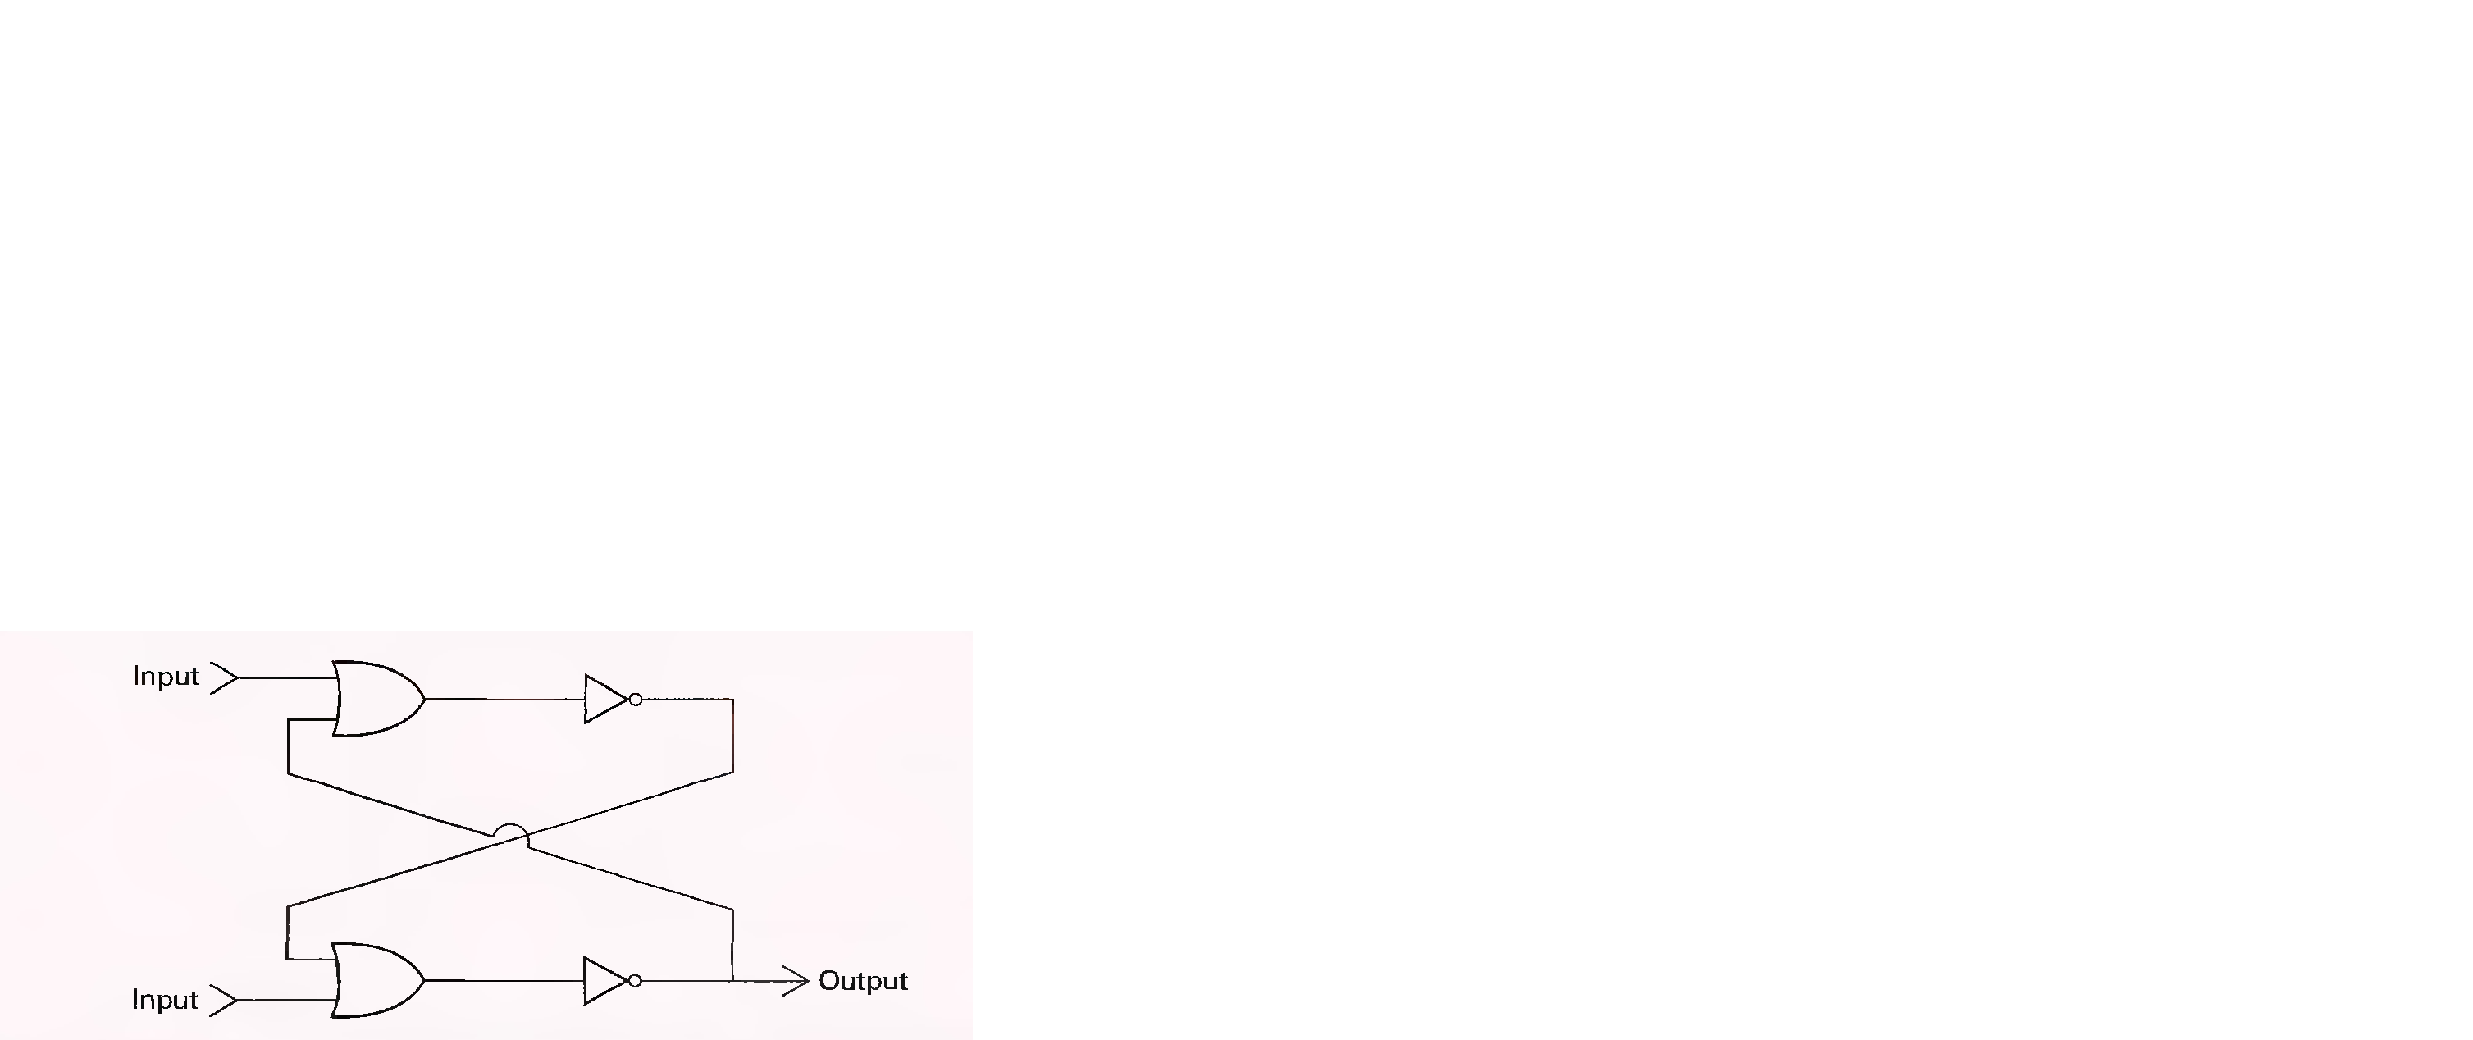
\includegraphics{ch2/fig15.pdf}}
   \end{center}


 \item Phối hợp các hoạt động của các thành phần khác nhau bên trong
   máy tính là rất cần thiết. Điều này được làm bằng cách nối với một
   xung đồng hồ với các mạch cần phối hợp.  Bởi vì đồng hồ thay đổi
   luân phiên giữa giá trị $0$ và $1$, nó làm cho các thành phần mạch
   hoạt động. Dưới đây là một ví dụ một phần của mạch liên quan đến
   Flip-Flop trong Hình~\ref{fig:op-flipflop}. Giá trị nào của xung
   đồng hồ sẽ chặn các giá trị đầu vào của mạch tác động đến
   Flip-Flop? Giá trị nào của xung đồng hồ sẽ làm cho Flip-Flop phản
   ứng lại với giá trị đầu vào của mạch?
    \begin{center}
      \scalebox{0.55}{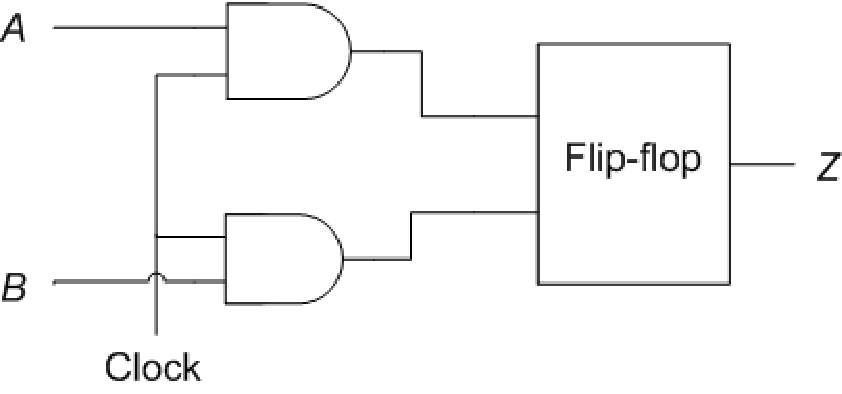
\includegraphics{ch2/bt4.pdf}}
    \end{center}

\item
  \begin{enumerate}
  \item Nếu đầu ra của cổng $\OR$ được nối với cổng $\NOT$, ta gọi nó
    là mạch $\NOR$. Mạch này có đầu ra là $1$ chỉ khi cả hai đầu vào
    đều có giá trị $0$. Ta ký hiệu cổng này cũng giống cổng $\OR$
    nhưng thêm một vòng tròn ở đầu ra của nó. Mạch dưới đây bao gồm
    một cổng $\AND$ và hai cổng $\NOR$. Hãy mô tả phép toán Boolean mà
    mạch này tính?
%\begin{figure}[h]
    \begin{center}
      \scalebox{0.55}{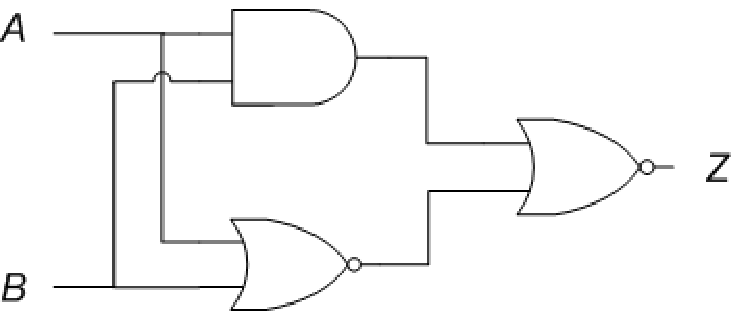
\includegraphics{ch2/bt5a.pdf}}
    \end{center}
%\caption{Một mạch Flip-Flop}
%  \label{fig:op-flipflop}
%\end{figure}

  \item Nếu đầu ra của cổng $\AND$ được nối với cổng $\NOT$, ta gọi nó
    là mạch $\NAND$.  Mạch này có đầu ra là $0$ chỉ khi cả hai đầu vào
    đều có giá trị $1$. Ta ký hiệu cổng này cũng giống cổng $\AND$
    nhưng thêm một vòng tròn ở đầu ra của nó. Mạch dưới đây bao gồm
    các cổng $\NAND$. Hãy mô tả phép toán Boolean mà mạch này tính?
    \begin{center}
      \scalebox{0.55}{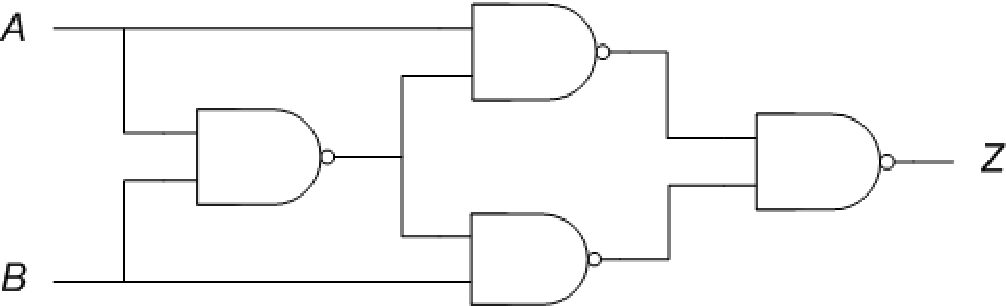
\includegraphics{ch2/bt5b.pdf}}
    \end{center}

  \end{enumerate}
\end{enumerate}

%%% Local Variables: 
%%% mode: latex
%%% TeX-master: "../tindaicuong"
%%% End: 
   
\section{Bộ nhớ chính}

Để lưu trữ dữ liệu, một máy tính chứa một tập các mạch (kiểu như Flip-Flops), mỗi mạch có
khả năng lưu trữ một bít. Dãy bít này gọi là \textbf{bộ nhớ chính} của máy.

\subsection*{Tổ chức bộ nhớ}
Bộ nhớ chính của máy tính được tổ chức theo các đơn vị dễ quản lý, gọi là các \textbf{ô
  nhớ}, một ô nhớ thường gồm tám bít (hay là một \textbf{byte}). Với các máy tính nhỏ dùng
cho các thiết bị gia đình như lò vi sóng, bộ nhớ chính của nó có thể chỉ gồm vài nghìn ô
nhớ. Trong khi các máy tính lớn có thể có bộ nhớ chính lên tới hàng tỷ ô nhớ.

Các ô nhớ trong máy tính không có thứ tự. Tuy nhiên, ta vẫn thường quy ước sắp xếp chúng
theo hàng. Phía phải nhất của hàng này được gọi là ở vị trí \textbf{cao} và phía trái được
gọi là vị trí \textbf{thấp}. Mỗi vị trí (byte) của hàng ta lại đánh thứ tự tính từ
\textit{phải qua trái}. Bít phía trái nhất có trọng số cao nhất và cũng thường được gọi là
\textbf{bít dấu} (cách gọi này dựa theo cách biểu diễn giá trị số của ô nhớ.).  Ta có thể
biểu diễn nội dung của ô nhớ với kích thước tính theo byte như theo Hình~\ref{fig:fig1.8}.

\begin{figure}[tb]
\centering
    \scalebox{0.4}{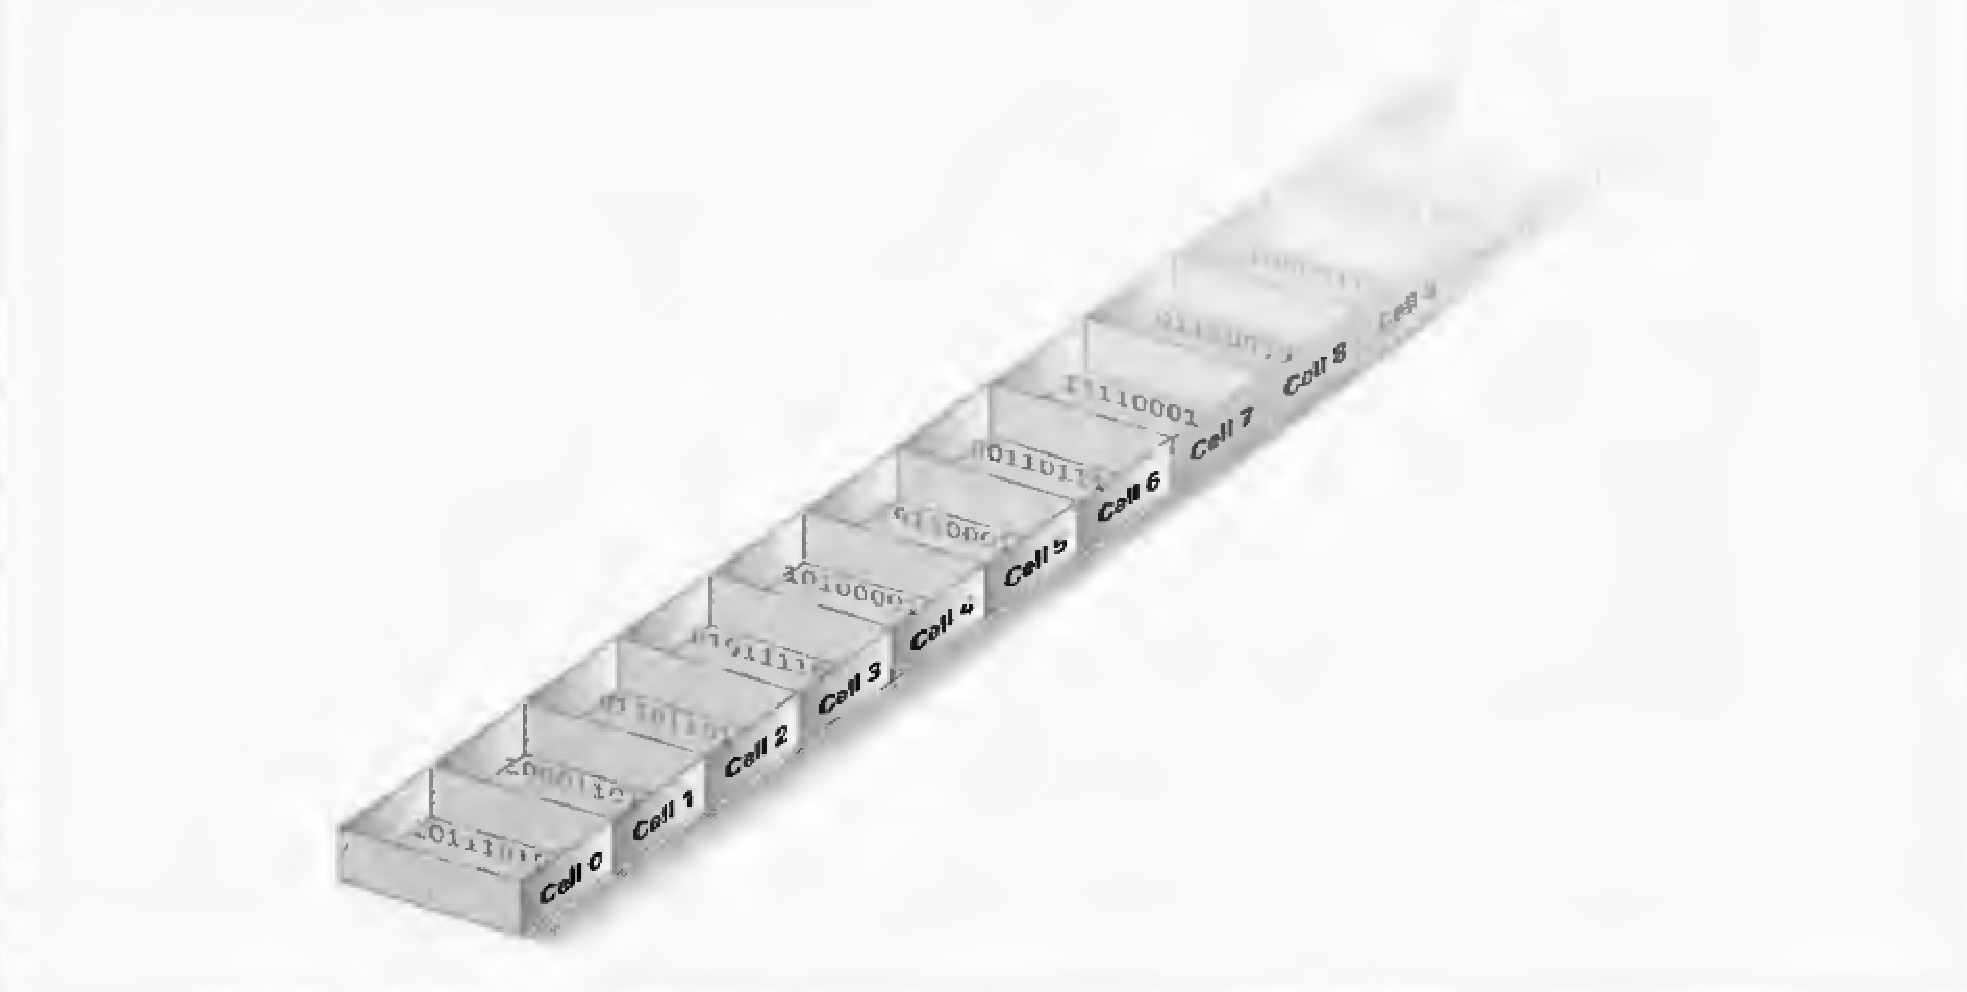
\includegraphics{ch2/Fig1-8.pdf}}
\caption{Các ô nhớ được sắp xếp theo địa chỉ}
  \label{fig:fig1.8}
\end{figure}

Để xác định ô nhớ trong bộ nhớ chính, mỗi ô nhớ được gán với một ``tên'' duy nhất, được
gọi là \textbf{địa chỉ}. Phương pháp này tương tự với cách đánh địa chỉ nhà trong thành
phố. Chính xác hơn, ta nhìn các ô nhớ xếp theo hàng và đánh số bắt đầu từ $0$. Cách đánh
địa chỉ kiểu này cho ta cách xác định ô nhớ một cách duy nhất. Tuy vậy, nó cũng gắn cho
các ô nhớ một thứ tự (Hình \ref{fig:fig1.8}), thứ tự này cho phép ta sử dụng các thuật ngữ ``ô
nhớ tiếp theo''  hoặc thuật ngữ ``ô nhớ trước''.


Việc gán thứ tự cho các ô nhớ trong bộ nhớ chính và các bít bên trong mỗi ô nhớ cho phép
ta đánh thứ tự các bít của  bộ nhớ chính theo hàng. Vậy ta có thể lưu trữ các
dãy bít có kích thước lớn hơn kích thước  của một ô nhớ. Ví dụ, ta có thể lưu trữ các xâu $16$ bít bằng hai ô nhớ liên tiếp.

% Để bổ trợ cho bộ nhớ chính, các mạch thực sự lưu trữ các bít được tổ
% hợp với mạch được yêu cầu để cho phép mạch lưu trữ và lấy dữ liệu từ
% các ô nhớ. Theo cách này, các mạch khác có thể lấy dữ liệu từ bộ nhớ
% bằng cách hỏi nội dung của một số ô nhớ (được gọi là thao tác đọc bộ
% nhớ), hoặc chúng có thể ghi thông tin vào trong bộ nhớ bằng cách yêu
% cầu một số bít đặt trong ô nhớ tại địa chỉ đặc biệt (được gọi là phép
% toán ghi).
%[.....]

Bởi vì bộ nhớ chính của máy tính được tổ chức như tập các ô nhớ riêng biệt được địa chỉ
hoá, nên các ô nhớ này có thể được truy cập một cách độc lập theo yêu cầu (cách truy cập
này của bộ nhớ chính ngược lại với cách truy cập của thiết bị lưu trữ khối, là thiết bị
trong đó các xâu bít dài được xử lý theo từng  khối). Để mô tả khả năng có thể
truy nhập được vào mọi ô nhớ, bộ nhớ chính được gọi là \textbf{bộ nhớ truy cập ngẫu nhiên
  (RAM)}.

Ta đã giới thiệu các Flip-Flop để lưu trữ các bít, nhưng trên thực tế bộ nhớ RAM trong
các máy tính hiện đại thường được xây dựng theo kỹ thuật khác. Kỹ thuật này cho phép bộ
nhớ có kích thước nhỏ hơn và có thời gian trả lời nhanh hơn. Thông thường, người ta dùng các  mạch điện nhỏ dễ  bị mất điện tích để lưu trữ các bít. Bởi vậy các thiết
bị này thường cần thêm các mạch, gọi là mạch làm tươi, chịu trách nhiệm nạp điện nhiều
lần một giây.

Để đoán nhận việc hay thay đổi này, bộ nhớ máy tính được xây dựng từ kiểu kỹ thuật này gọi là
bộ nhớ động, dẫn tới thuật ngữ \textbf{DRAM} (Dynamic RAM). Hoặc, tại thời điểm viết quyển
sách này, người ta hay nói tới \textbf{SDRAM} (Synchronous DRAM, có nghĩa rằng DRAM có sử
dụng kỹ thuật đồng bộ (Synchronous) làm giảm thời gian cần thiết để lấy nội dung của một ô
nhớ.)

\subsection*{Đơn vị đo khả năng bộ nhớ}
Ta sẽ thấy trong chương tiếp theo rằng việc thiết kế hệ thống bộ nhớ chính trong đó tổng
số ô nhớ là một luỹ thừa của $2$ có rất nhiều điểm tiện lợi. Kích thước của bộ nhớ trước
đây thường được tính theo $1024$ (bằng $2^{10}$) đơn vị ô nhớ. Bởi vì $1024$ là gần với
giá trị $1000$, người ta thường sử dụng tiền tố \textit{kilo} cho đơn vị này. Có nghĩa
rằng, thuật ngữ \textit{kilobyte} (viết tắt là KB) được sử dụng để chỉ $1024$ byte. Bởi
vậy, một máy với $4096$ ô nhớ được gọi là có $4$KB bộ nhớ ($4096 = 4 \times 1024$). Khi bộ
nhớ trở nên lớn hơn, thuật ngữ này được phát triển thêm bao gồm các tiền tố \textit{mega}
cho $1,048,576$ (bằng $2^{20}$) và \textit{giga} cho $1,073,741,824$ (bằng $2^{30}$), và
đơn vị như MB (megabyte) và GB (gigabyte) trở nên phổ biến.

Không may, việc áp dụng các tiền tố thể hiện đơn vị tính có thể gây nhầm lẫn vì các tiền
tố này đã được sử dụng trong các lĩnh vực khác theo đơn vị đo là luỹ thừa của~$10$. Ví dụ,
khi tính khoảng cách, một \textit{kilo-mét} tương ứng bằng $1000$ mét, và khi đo tần xuất
radio, một \textit{mega-hertz} tương ứng bằng $1,000,000$ hertz. Tình huống còn tệ hơn khi
một số nhà sản xuất thiết bị máy tính còn pha trộn hai kiểu thuật ngữ này, dùng KB để
chỉ~$1024$ byte nhưng MB theo nghĩa là $1000$KB (bằng $1,024,000$ byte). Điều này gây lộn
xộn và không rõ ràng cho người dùng thuật ngữ này.

Để làm rõ ràng, người ta đề nghị dùng tiền tố \textit{kilo, mega}, và \textit{giga} cho
các đơn vị theo luỹ thừa của~$10$, và đưa thêm các tiền tố mới \textit{kibi} (viết tắt
kilobinary và ký hiệu là Ki), \textit{mebi} (viết tắt cho megabinary và ký hiệu là Mi), và
\textit{gibi} (viết tắt cho gigabinary và ký hiệu là Gi) tương ứng với đơn vị theo luỹ
thừa của $2$. Với hệ thống này, thuật ngữ \textit{kibibyte} (KiB) có thể để chỉ $1024$
byte, trong khi đó \textit{kilobyte} (KB) dùng để chỉ $1000$ byte. Các thuật ngữ này có
trở thành phổ biến hay không thì phải chờ thời gian trả lời. Hiện tại các thuật ngữ bị
hiểu nhầm \textit{kilo, mega,} và \textit{giga} vẫn bị ăn sâu trong cộng đồng người sử
dụng khi nói tới bộ nhớ chính, bởi vậy ta vẫn theo các ký hiệu truyền thống trong các
nghiên cứu khi tham khảo đến việc lưu trữ dữ liệu. Tuy vậy, các tiền tố \textit{kibi,
  megi}, và \textit{gibi} được đưa ra nhằm giải quyết vấn đề này, và có thể rằng là khôn
ngoan khi diễn dịch các thuật ngữ như \textit{kilobyte} và \textit{megabyte} kèm theo lời
cảnh báo.

\subsection*{Câu hỏi \& Bài tập}
\begin{enumerate}
\item Nếu ô nhớ số $5$ chứa giá trị $8$, hãy chỉ ra sự khác nhau giữa việc viết
  giá trị~$5$ vào ô nhớ số $6$ và chuyển nội dung của ô nhớ số $5$ vào ô nhớ số $6$?

\item Giả sử rằng bạn muốn hoán đổi các giá trị được lưu trữ tại ô nhớ số $2$ cho ô nhớ số
  $3$. Cách thực hiện sau đây có gì sai:
  \begin{description}
  \item \textit{Bước 1.} Chuyển nội dung của ô nhớ số $2$ vào ô nhớ số $3$.
  \item \textit{Bước 2.} Chuyển nội dung của ô nhớ số $3$ vào ô nhớ số $2$.
  \end{description}
  Thiết kế một dãy các bước thực hiện đúng việc tráo đổi nội dung của hai ô nhớ này.

\item Có thể lưu trữ bao nhiêu bít vào bộ nhớ máy tính có dung lượng $4$KB (chính xác hơn
  là KiB)?
  
\end{enumerate}
\section{Thiết bị lưu trữ khối}

Do tính không bền vững và kích thước hạn chế của bộ nhớ chính, nên hầu hết các máy tính
đều có thêm thiết bị nhớ,  gọi là các hệ thống lưu trữ khối (hoặc là lưu trữ thứ
cấp). Các thiết bị này bao gồm đĩa từ, CD, DVD, băng từ, và ổ đĩa flash (ta sẽ thảo luận
các thiết bị này sau). Ưu điểm của hệ thống lưu trữ khối so với bộ nhớ chính là tính lưu
trữ thông tin lâu dài, khả năng lưu trữ lớn, giá thành thấp, và trong nhiều trường hợp cho
ta khả năng có thiết bị lưu trữ tạm thời có thể tách rời khỏi máy.

Thuật ngữ \textit{on-line} và \textit{off-line} thường được sử dụng để mô tả thiết bị được
gắn hoặc tách rời khỏi máy. \textbf{On-line} có nghĩa rằng thiết bị hoặc thông tin được
kết nối và sẵn sàng để đọc từ máy mà không cần sự can thiệp của con
người. \textbf{Off-line} có nghĩa rằng cần sự can thiệp của con người trước khi thiết bị
hoặc thông tin có thể truy cập được từ máy--có thể bởi vì thiết bị phải được bật, hoặc cơ
cấu làm việc yêu cầu các thông tin trung gian phải được thêm vào.

Điểm bất lợi chính của thiết bị lưu trữ khối yêu cầu các dịch chuyển cơ học và bởi thế
chúng cần nhiều thời gian hơn để lưu trữ và nhận dữ liệu từ máy so với bộ nhớ chính, nơi
mà mọi hoạt động đều được thực hiện bằng điện.

\subsection*{Các hệ thống từ tính}


Theo thời gian, các công nghệ từ đang chiếm ưu thế trong lĩnh vực lưu trữ khối. Ví dụ, thiết bị  điển hình được  sử dụng ngày nay là \textbf{đĩa từ}, gồm các đĩa tròn được phủ từ được dùng để lưu trữ dữ liệu. Các đầu đọc/ghi được đặt ở trên và/hoặc dưới đĩa, và khi đĩa xoay tròn,
mỗi đầu đọc đi theo một vòng tròn, gọi là một \textbf{track}, quanh bề mặt bên trên và bên
dưới của đĩa. Bằng cách đặt lại vị trí của đầu đọc/ghi, ta có thể truy cập vào các track đồng tâm khác nhau. Trong nhiều trường hợp, hệ thống lưu trữ bao gồm một vài đĩa được gắn
với một ống suốt chung, đĩa này đặt trên đĩa khác, và khe nhỏ ở giữa hai đĩa đủ đặt các
đầu đọc/ghi. Các đầu đọc/ghi dịch chuyển theo cách thống nhất. Mỗi lần đầu đọc/ghi đặt
lại vị trí, ta lại có một tập mới các track, được gọi là \textbf{cylinder}, có thể truy
cập vào được.

Bởi vì một track thường chứa nhiều thông tin  hơn số thông tin ta muốn xử lý tại một thời điểm,
nên ta lại chia nhỏ mỗi track thành các cung, gọi là \textbf{sector}. Thông tin trên
các sector này được ghi như các xâu bít liên tục (Hình \ref{fig:fig1.9}). Các sector trên
một đĩa có thể có cùng số bít (thông thường là nằm trong khoảng từ $512$ byte tới một
KB). Trong trường hợp đơn giản nhất, hệ thống lưu trữ đĩa có số sector trên mỗi track là
bằng nhau. Vì các track bên ngoài có chu vi lớn hơn so với các track ở bên trong, nên
trong trường hợp này số bít trong một sector trên track ở phía ngoài của đĩa lưu trữ ít
dày đặc hơn so với các track ở gần trung tâm. Trên thực tế, với những hệ thống đĩa có khả
năng lưu trữ cao, các track ở phía ngoài xa trung tâm thường chứa nhiều sector hơn track ở
gần trung tâm. Ta có được khả năng này là nhờ áp dụng một kỹ thuật gọi là
\textbf{zoned-bit recording}. Dùng zone-bit recording, một vài track kề nhau được tập hợp
thành một vùng, các đĩa điển hình chứa khoảng mười vùng. Mọi track trong một vùng có cùng
số sector, nhưng các vùng bên ngoài có nhiều sector trên một track so với vùng bên trong
nó. Theo cách này, không gian lưu trữ của đĩa được sử dụng hiệu quả hơn so với cách của hệ
thống đĩa truyền thống. Nói một cách đơn giản, đây là một hệ thống lưu trữ bao gồm nhiều
sector riêng, mỗi sector có thể được truy cập như một xâu bít độc lập.

\begin{figure}[tb]
\centering
    \scalebox{0.3}{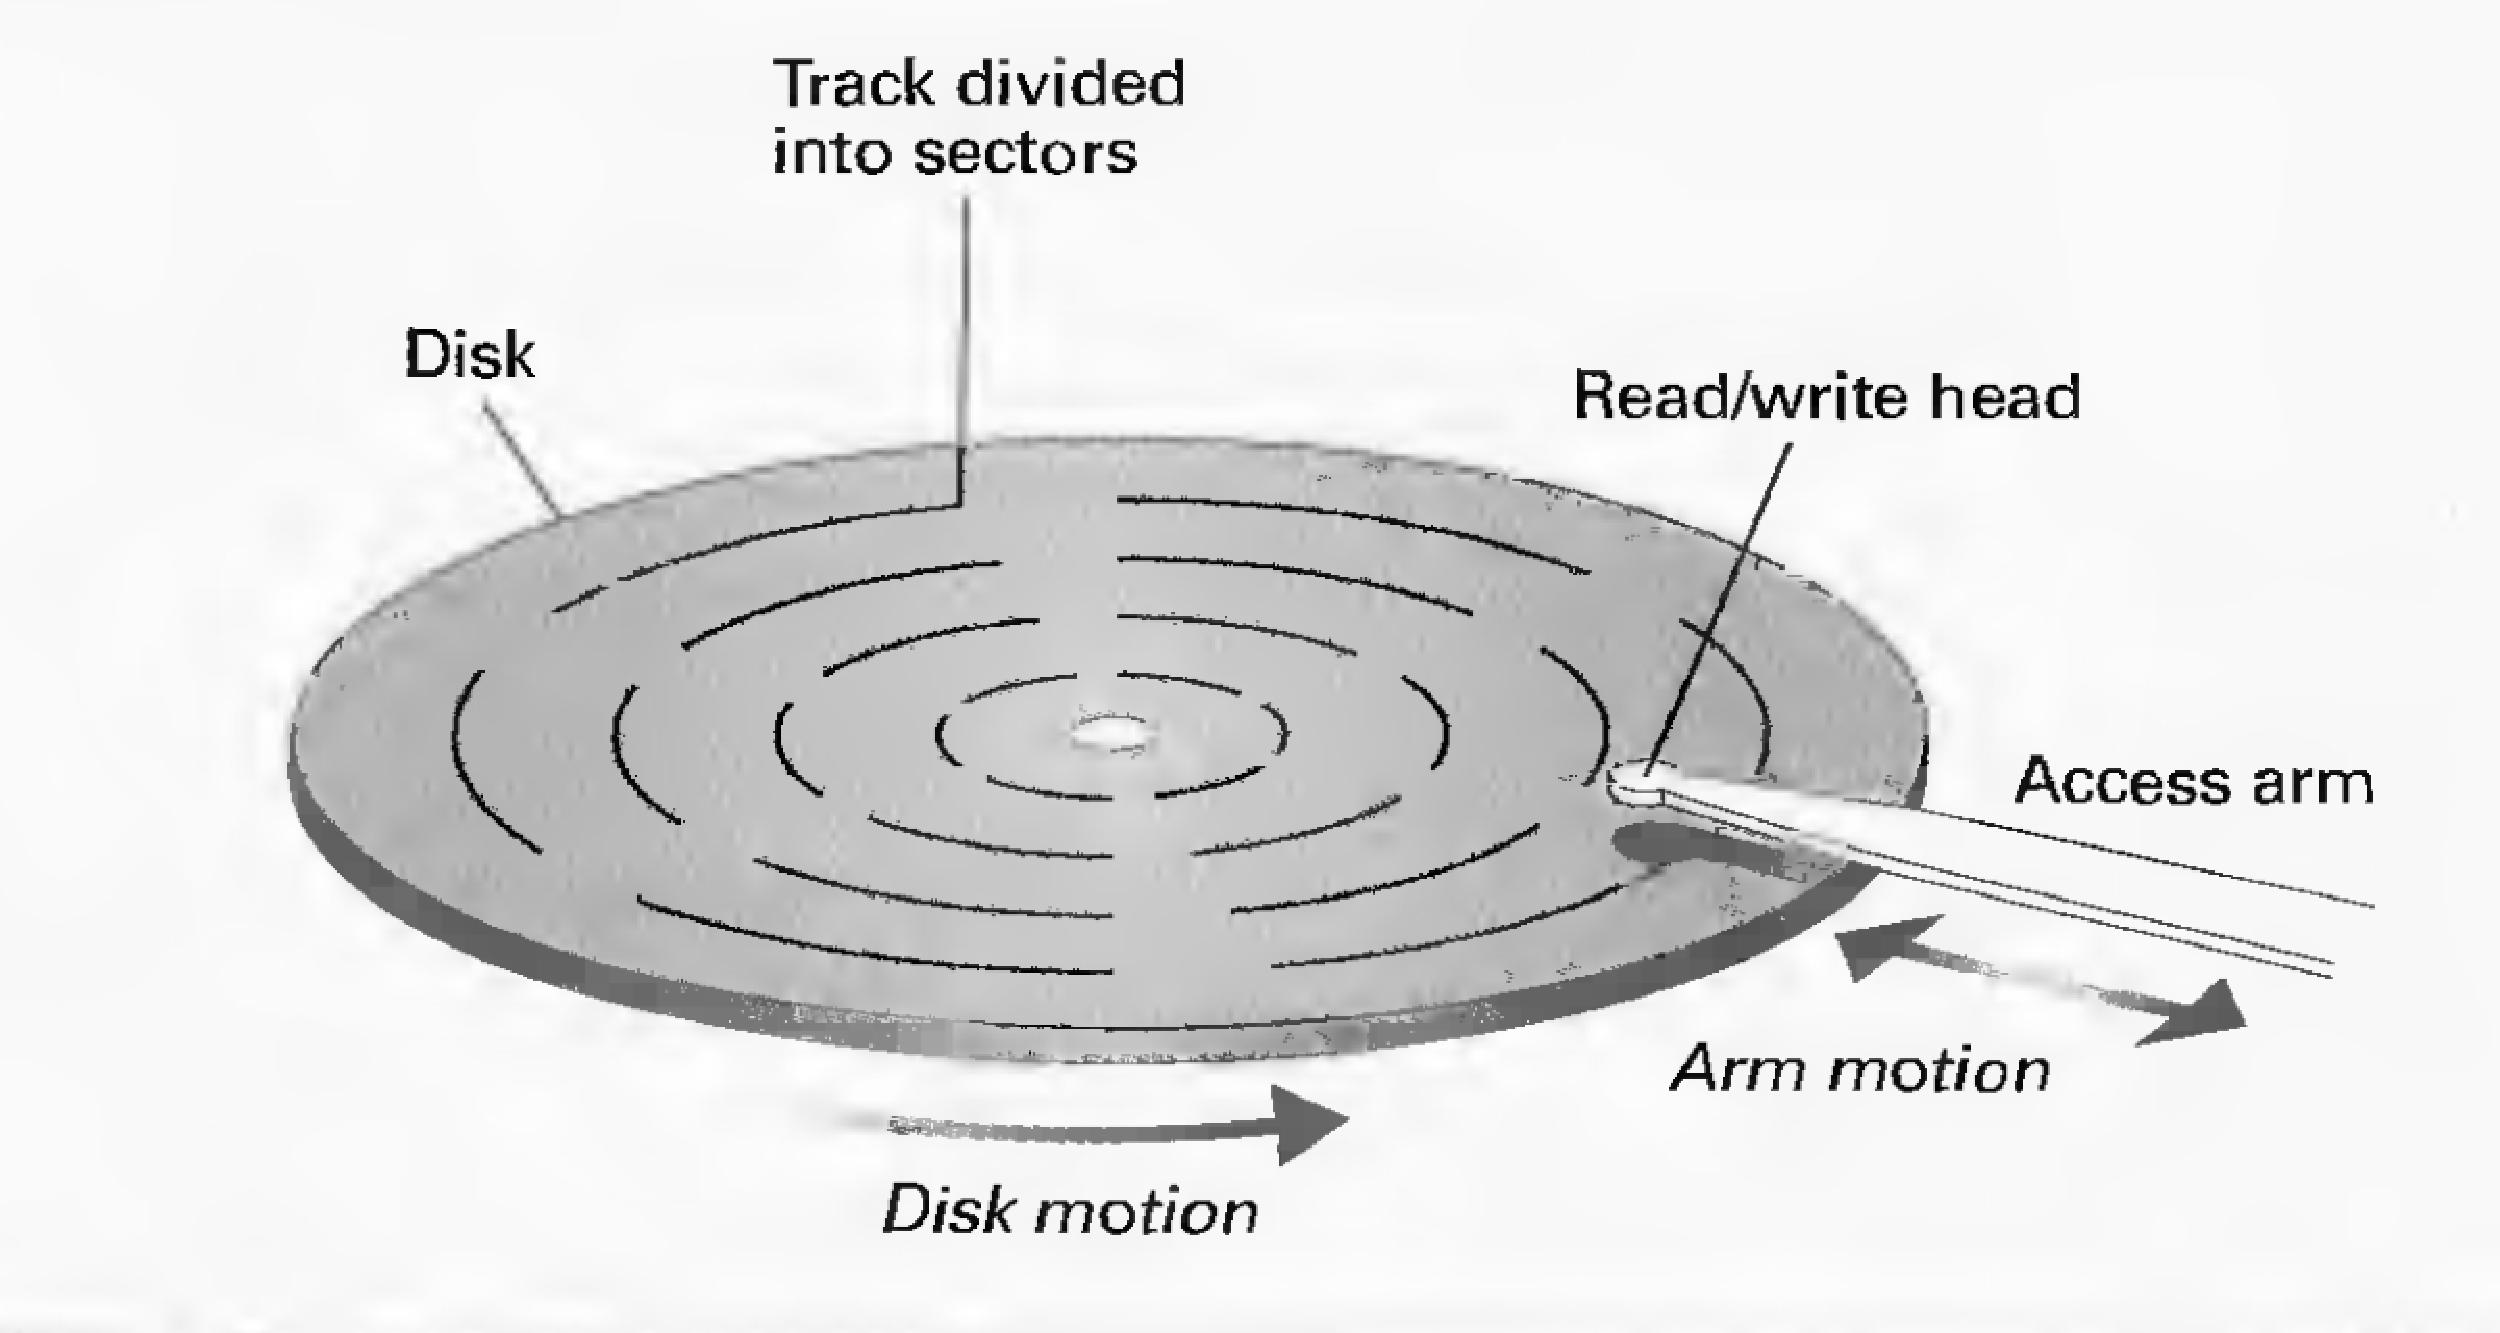
\includegraphics{ch2/Fig1-9.pdf}}
\caption{Một hệ thống lưu trữ đĩa}
  \label{fig:fig1.9}
\end{figure}

Vị trí các track và sector là có thể thay đổi so với cấu trúc vật lý
đĩa. Chúng được đánh dấu về mặt từ tính qua một quá trình gọi là \textbf{formating} (hay
khởi tạo) đĩa. Quá trình này thường được thực hiện bởi nhà sản xuất đĩa, kết quả ta được
một đĩa đã được format. Tuy vậy, hầu hết hệ thống máy tính đều có thể thực hiện nhiệm vụ
này. Bởi vậy, nếu thông tin format trên đĩa bị hỏng, đĩa có thể được format lại. Tuy nhiên
quá trình này sẽ phá huỷ mọi mọi thông tin đã được lưu trữ ghi trên đĩa trước đó.

Khả năng của hệ thống lưu trữ đĩa phụ thuộc vào số đĩa được sử dụng và mật độ track và
sector được thiết đặt. Các hệ thống mức thấp chỉ gồm một đĩa được làm bằng chất dẻo, gọi là \textbf{đĩa mềm}, hay bởi một tên ít dùng hơn là \textbf{floppy}. Đĩa mềm dễ đưa
vào và lấy ra từ các ổ đọc/ghi, đồng thời dễ được lưu trữ lại. Vậy nên đĩa mềm được
dùng rất phổ biến như thiết bị lưu trữ thông tin off-line. Tuy nhiên, bởi vì đĩa
mềm~$3\frac{1}{2}$-in chỉ có khả năng lưu trữ $1.44$MB, nên nó đã nhanh chóng
bị thay thế bởi công nghệ khác.

Các hệ thống đĩa có khả năng lưu trữ cao có thể lưu trữ lên tới nhiều gigabyte. Chúng có
thể bao gồm năm đến mười đĩa cứng đặt trên cùng một trục. Do các đĩa này được làm bằng
chất liệu cứng nên chúng thường được gọi là hệ thống đĩa cứng, ngược lại với thuật ngữ đĩa
mềm. Để cho phép tốc độ quay nhanh, các đầu đọc/ghi trong các hệ thống này không chạm vào
đĩa mà chỉ ``lơ lửng'' trên bề mặt đĩa. Không gian dành cho đầu đọc ở giữa hai đĩa là rất
hẹp, thậm chí chỉ một ít bụi cũng có thể làm kẹt đầu đọc và bề mặt đĩa, dẫn đến phá huỷ cả
hai (hiện tượng này gọi là vỡ đầu đọc). Bởi vậy nên các hệ thống đĩa cứng thường được đặt
bên trong case máy tính và được đóng kín bởi nhà sản xuất.

% Có một vài độ đo để đánh giá hiệu năng hệ thống đĩa:
% \begin{inparaenum}
% \item[(1)] \textbf{thời gian di chuyển} (thời gian chuyển đầu đọc từ track
%   này sang track khác).
% \item[(2)] \textbf{độ trễ vòng quay} hay \textbf{thời gian trễ}
% \end{inparaenum}

%[....]

Hệ thống đĩa cứng nói chung có những đặc trưng tốt hơn so với đĩa mềm. Bởi vì đầu đọc/ghi
không chạm vào bề mặt đĩa, nên nó có tốc độ quay lên tới vài nghìn vòng trong một
phút. Trong khí đó hệ thống đĩa mềm quay chỉ khoảng $300$ vòng một phút. Do đó tốc độ
truyền của hệ thống đĩa cứng, thường là vài MB trên giây, lớn hơn rất nhiều so với đĩa mềm
(chỉ vài KB trên giây).

Do các thao tác của hệ thống đĩa yêu cầu chuyển động về mặt vật lý, nên nó kém hơn rất
nhiều so với tốc độ của mạch điện tử. Thời gian trễ của mạch điện được tính theo đơn vị
nano giây (một phần tỷ của giây) hoặc ít hơn, trong khi đó thời gian di chuyển, thời gian
trễ và thời gian truy cập của hệ thống đĩa được tính theo mili-giây (một phần nghìn của
giây). Bởi vậy, khi các mạch điện đợi lấy kết quả từ hệ thống đĩa, thời gian dường như là
vô tận.

Không chỉ có hệ thống lưu trữ đĩa là thiết bị lưu trữ khối dùng công nghệ từ. Một dạng cũ
hơn của lưu trữ khối dùng công nghệ từ là \textbf{băng từ} (Hình \ref{fig:fig1.10}). Trong
các hệ thống này, thông tin được ghi dưới dạng một băng mềm mỏng quấn xung quanh một ống
để lưu trữ.
 
%[.....]

\begin{figure}[bth]
  \centering \scalebox{0.4}{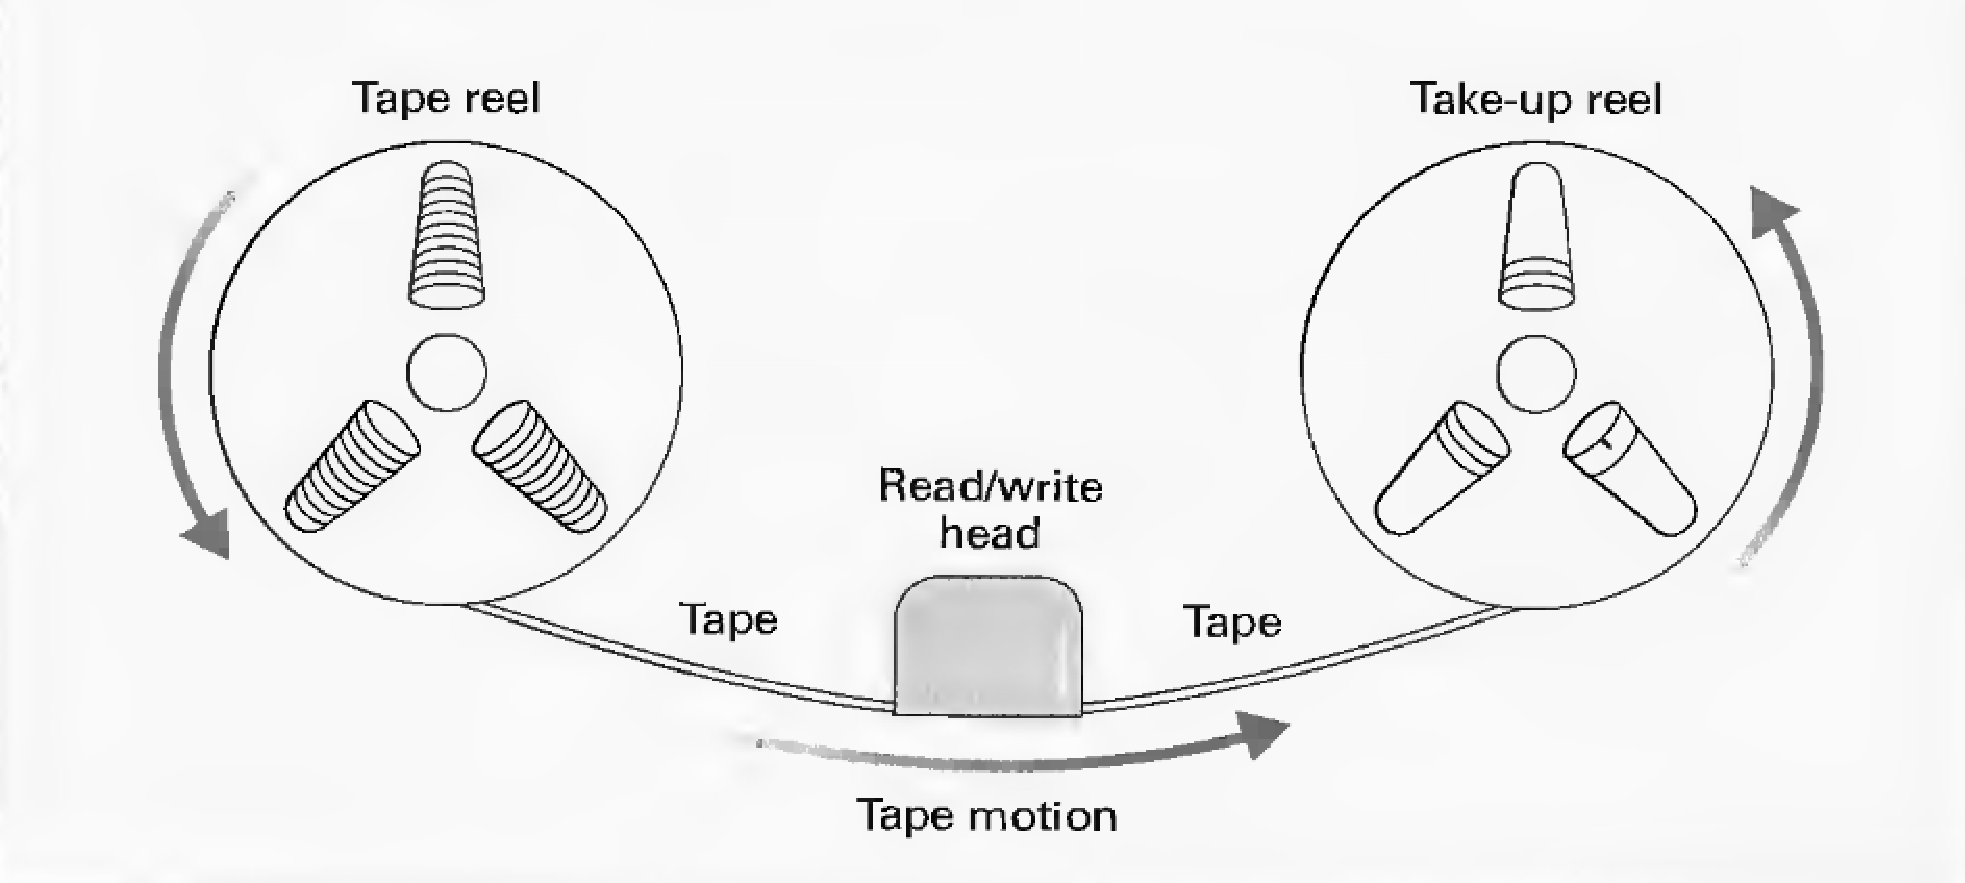
\includegraphics{ch2/Fig1-10.pdf}}
\caption{Cơ chế lưu trữ băng từ}
  \label{fig:fig1.10}
\end{figure}

\subsection*{Hệ thống quang}

Có một lớp thiết bị lưu trữ khối áp dụng kỹ thuật quang. Ví dụ đĩa \textbf{CD} (Compact
Disk). Các đĩa này có đường kính là $12$cm (xấp xỉ $5$ inches) và được phủ một lớp gương
với một lớp phủ bảo vệ. Thông tin được ghi trên đĩa bằng cách thay đổi bề mặt phản xạ. Vì
vậy, các thông tin này có thể được lưu trữ theo cách chùm tia laser được phóng không theo
quy luật trên bề mặt phản xạ của CD khi nó quay.

Công nghệ CD đã được ứng dụng trước đây cho việc thu âm dùng định dạng quen thuộc như
\textbf{CD-DA} (Compact disk-digital audio). Các đĩa CD sử dụng ngày nay về cơ bản có cùng
định dạng. Cụ thể, các thông tin trên các đĩa CD được lưu trữ trên một track đơn xoắn ốc
xung quanh CD giống cách ghi cũ, tuy nhiên điểm khác biệt là các track trên đĩa CD xoắn ốc
theo chiều từ trong ra~(Hình \ref{fig:fig1.11}). Track này được chia thành các đơn vị gọi
là sector, mỗi sector có định danh riêng của nó và có khả năng lưu giữ $2$KB dữ liệu,
tương đương với $\frac{1}{75}$ giây âm nhạc trong trường hợp ghi âm.
 
\begin{figure}[bth]
\centering
    \scalebox{0.3}{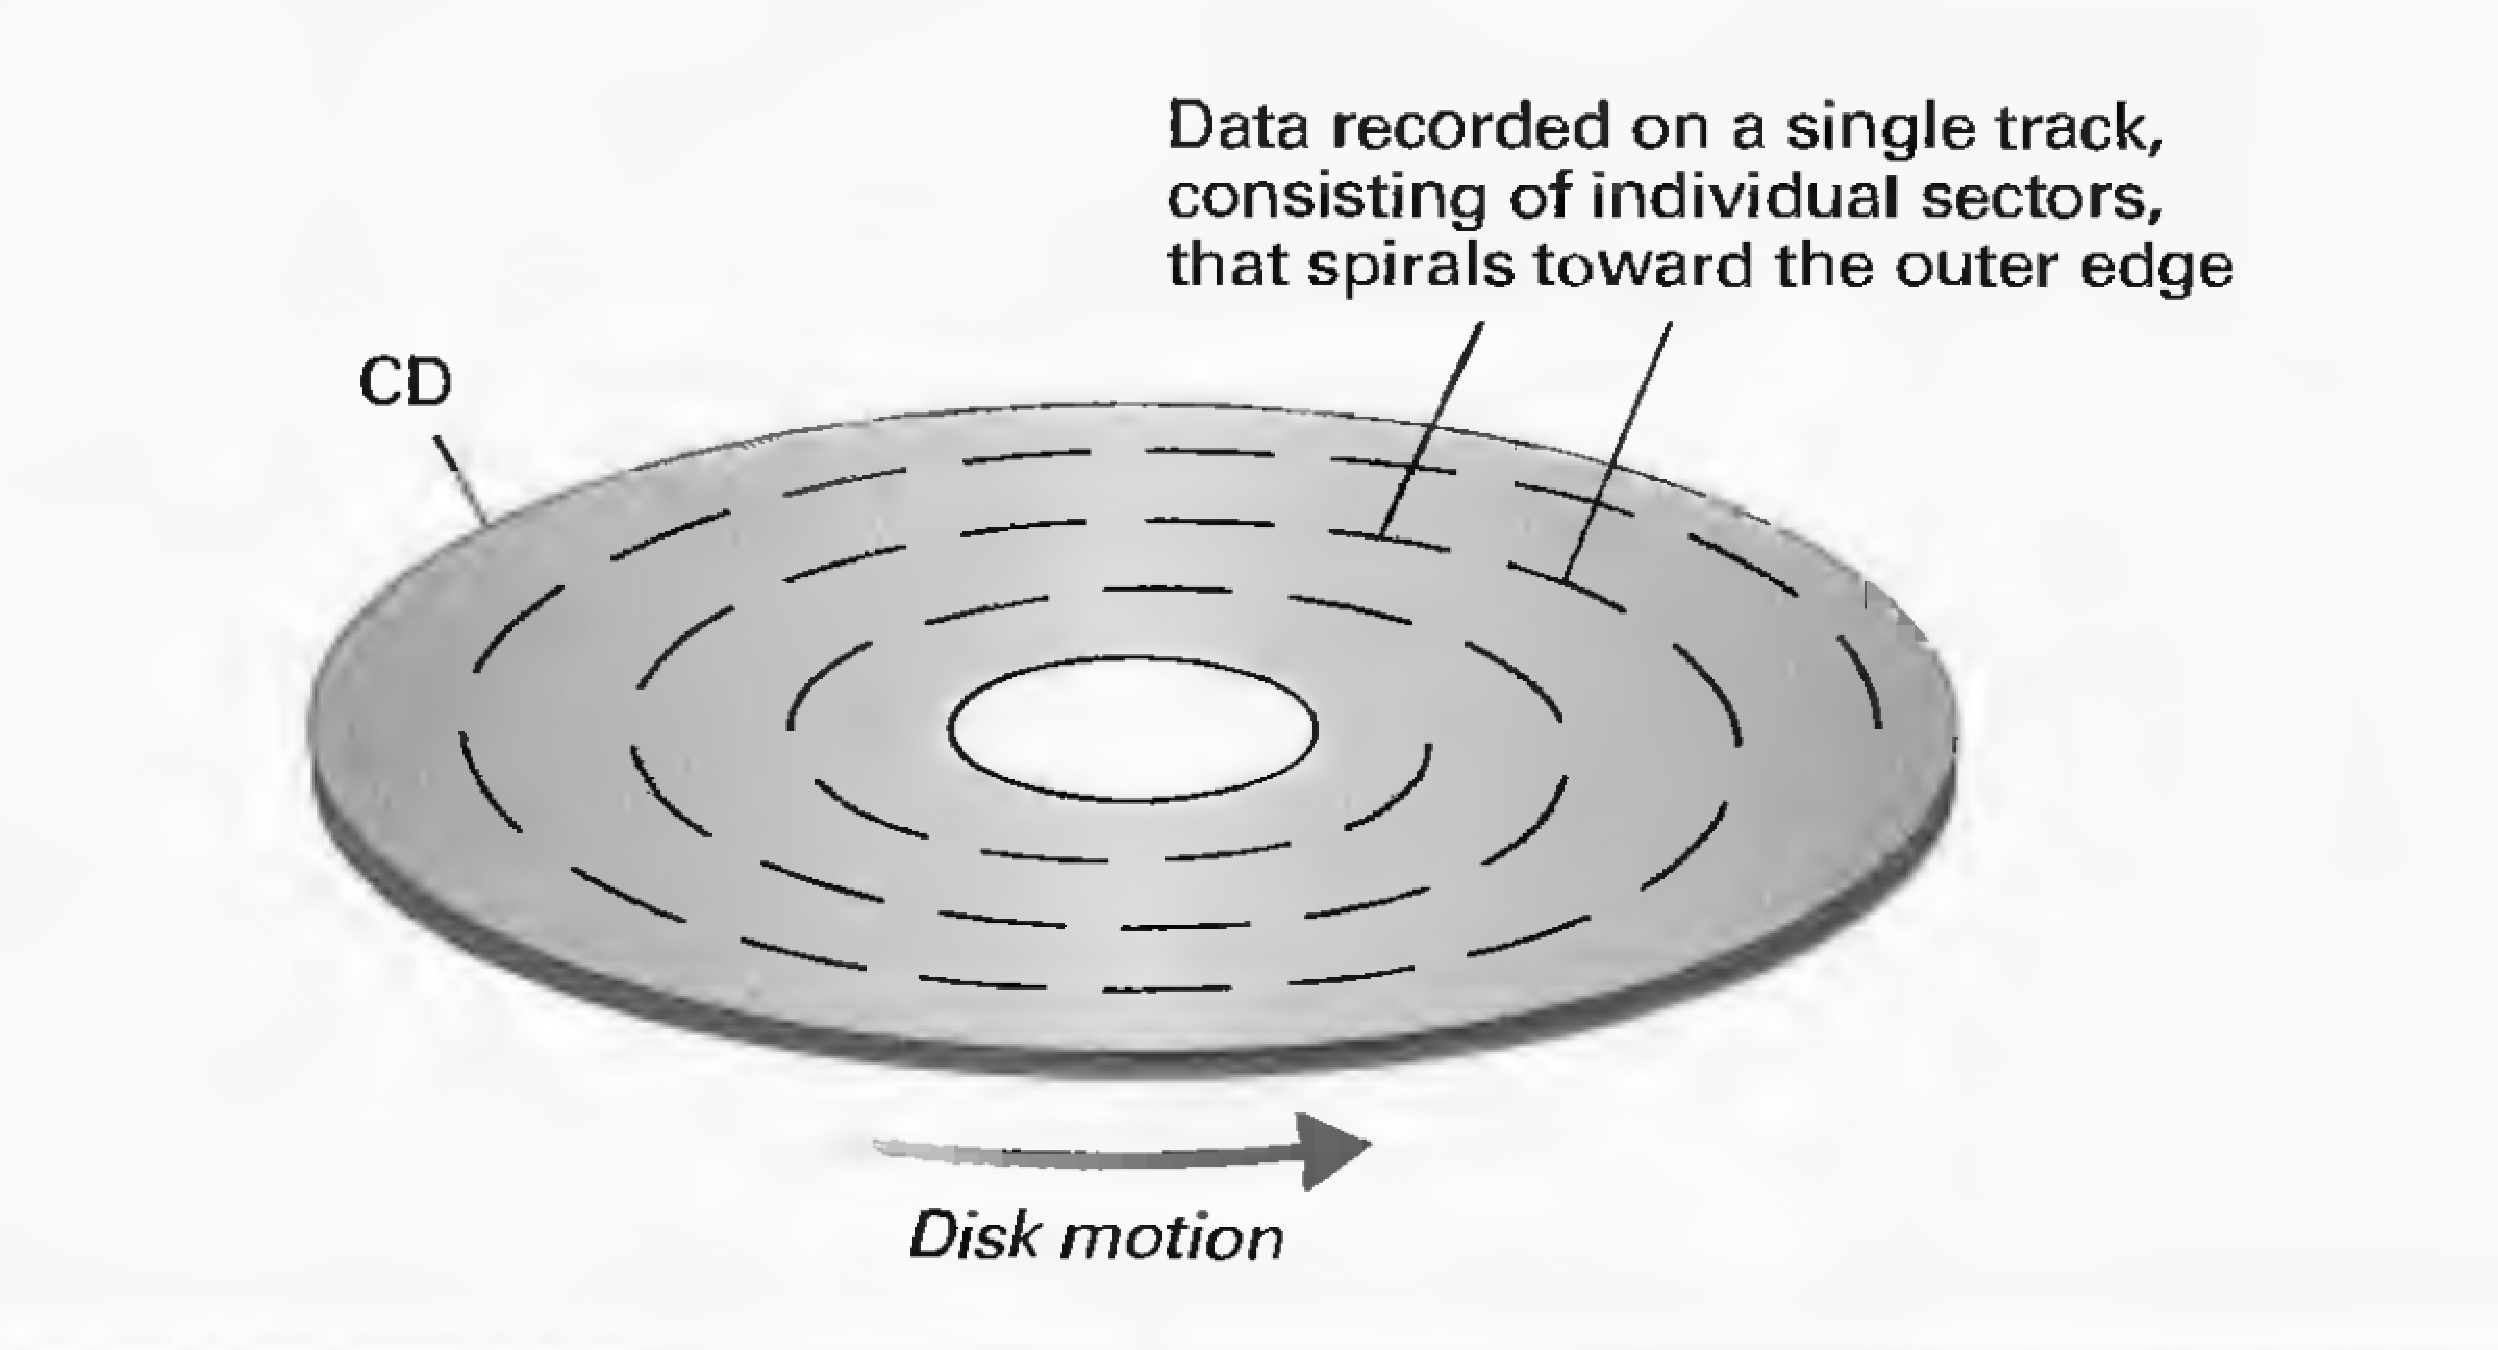
\includegraphics{ch2/Fig1-11.pdf}}
\caption{Định dạng lưu trữ của CD}
  \label{fig:fig1.11}
\end{figure}


% Chú ý rằng khoảng cách quanh track xoắn ốc là lớn dần từ trong ra
% ngoài. Để có thể có khả năng tốt nhất của một CD, các thông tin được
% lưu trữ theo mật đô phân phối tuyến tính chuẩn trên toàn bộ 

%[....]

Như một hệ quả của cách thiết kế, các hệ thống lưu trữ CD thực hiện tốt nhất với xâu dữ
liệu liên tục, dài, giống như khi sản xuất âm nhạc. Ngược lại, khi ứng dụng yêu cầu truy
cập ngẫu nhiên, cách tiếp cận dùng đĩa từ (gồm các track đồng tâm được chia thành các
sector có thể truy cập riêng biệt) làm tốt hơn cách tiếp cận xoắn ốc được dùng trong CDs.

Các đĩa CD truyền thống có khả năng lưu trữ $600$ đến $700$MB. Tuy nhiên, những đĩa
\textbf{DVD (Digital Versatile Disk)}, được xây dựng từ nhiều mối phức tạp, các tầng nửa
trong suốt phục vụ như bề mặt phân biệt khi được nhìn bởi một tia laser hội tụ một cách
chính xác, cho phép khả năng lưu trữ lên tới vài GB. Kiểu đĩa như thế này có khả năng lưu
trữ trình diễn đa phương tiện dài, bao gồm cả hình ảnh chuyển động.

\subsection*{Thiết bị Flash}

Một tính chất chung của thiết bị lưu trữ khối dựa trên công nghệ từ hoặc quang là chuyển
động vật lý như các đĩa xoay, di chuyển đầu đọc, và bắn chùm tia laser, được yêu cầu để
lưu trữ và lấy dữ liệu. Điều này có nghĩa rằng việc lưu trữ dữ liệu và tìm kiếm là chậm so
với mạch điện tử. Công nghệ \textbf{bộ nhớ flash} có khả năng giúp giảm bớt hạn chế
này. Trong hệ thống nhớ flash, các bít được lưu trữ bằng cách gửi tín hiệu điện trực tiếp
tới môi trường lưu trữ ở đó các electron được giữ trong một khoang nhỏ chứa silicon
dioxide, bởi vậy nó biến đổi các đặc trưng của mạch điện. Bởi vì các khoang chứa này có
khả năng giữ các electron trong nhiều năm, nên công nghệ này có thể phù hợp cho việc lưu
trữ dữ liệu off-line.

Mặc dù dữ liệu được lưu trữ trong hệ thống bộ nhớ flash có thể được truy cập theo đơn vị
kích thước nhỏ tính theo byte giống như trong ứng dụng RAM, nhưng hạn chế của công nghệ
hiện nay khiến cho dữ liệu phải được lưu trữ xoá theo khối lớn. Hơn nữa lặp lại việc xoá
sẽ gây thiệt hại cho khoang chứa silicon dioxide. Hạn chế này làm cho công nghệ bộ nhớ
flash hiện tại không thích hợp cho các ứng dụng bộ nhớ chính, nơi yêu cầu nội dung phải
thay đổi nhiều lần trong một giây. Tuy nhiên, đối với các ứng dụng mà tính thay đổi có thể
được điều chỉnh ở mức độ hợp lý như camera số, điện thoại di động, máy PDA cầm tay, thì bộ
nhớ flash lại trở thành thiết bị lưu trữ khối được lựa chọn. Thật vậy, bởi vì bộ nhớ flash
không nhạy cảm với các va chạm về mặt vật lý (ngược lại với hệ thống từ và quang) nên tiềm
năng của nó với các ứng dụng di động là rất hấp dẫn.

Các thiết bị flash được gọi là \textbf{flash drives}, với khả năng lên tới vài GB, là sẵn
có cho các ứng dụng lưu trữ khối tổng quát. Các đơn vị này được nén trong miếng nhựa nhỏ
có độ dài xấp xỉ ba inche cùng với nắp bảo vệ đơn vị kết nối điện khi thiết bị
off-line. Khả năng cao của các đơn vị di động này cũng như sự kiện rằng chúng dễ kết nối
và ngắt kết nối từ máy tính làm cho chúng trở thành lý tưởng cho việc lưu trữ dữ liệu
off-line. Tuy nhiên, tính dễ tổn thương của khoang lưu trữ làm cho chúng không tin cậy như
đĩa quang cho việc lưu trữ thực sự lâu dài.

\subsection*{Lưu trữ và tìm kiếm file}

Thông tin được lưu trữ trong hệ thống lưu trữ khối về mặt thiết kế được nhóm lại thành các
đơn vị lớn gọi là \textbf{file}. Một file điển hình có thể là một tài liệu văn bản được
hoàn thành, một tấm ảnh, một chương trình, một đĩa nhạc, hoặc một tập dữ liệu về nhân viên
trong công ty. Ta đã thấy rằng thiết bị lưu trữ khối làm cho các file được lưu trữ ít
hơn. Ví dụ, một file được lưu trữ trên một đĩa từ phải được xử lý theo sector, mà mỗi
sector có kích thước xác định trước. Một khối dữ liệu phù hợp với đặc trưng của thiết bị
lưu trữ được gọi là \textbf{bản ghi vật lý}. Bởi vậy, một file lớn được lưu trữ trong
thiết bị lưu trữ khối nói chung sẽ bao gồm nhiều bản ghi vật lý.

Ngược lại với cách chia theo các bản ghi vật lý này, một file thường phân chia tự nhiên
theo thông tin được biểu diễn. Ví dụ, một file chứa thông tin về nhân viên trong một công
ty có thể bao gồm nhiều đơn vị, mỗi đơn vị chứa thông tin về một nhân viên. Hoặc một file
chứa tài liệu văn bản có thể bao gồm nhiều đoạn hoặc trang văn bản. Các khối dữ liệu xuất
hiện tự nhiên như thế này được gọi là \textbf{các bản ghi logic}.


Các bản ghi logic thường bao gồm các đơn vị nhỏ hơn gọi là các \textbf{trường}. Ví dụ, một
bản ghi logic chứa thông tin về nhân viên có thể bao gồm trường tên, địa chỉ, số chứng
minh của nhân viên,... Đôi khi mỗi bản ghi logic trong một file xác định một cách duy nhất
bởi một trường đặc biệt bên trong bản ghi (có thể là số chứng minh thư của nhân viên, một
số, hoặc chỉ mục trong bảng liệt kê). Trường xác định như thế này được gọi là
\textbf{trường khoá}. Giá trị giữa trong trường khoá được gọi là \textbf{khoá}.
\begin{figure}
\centering
    \scalebox{0.3}{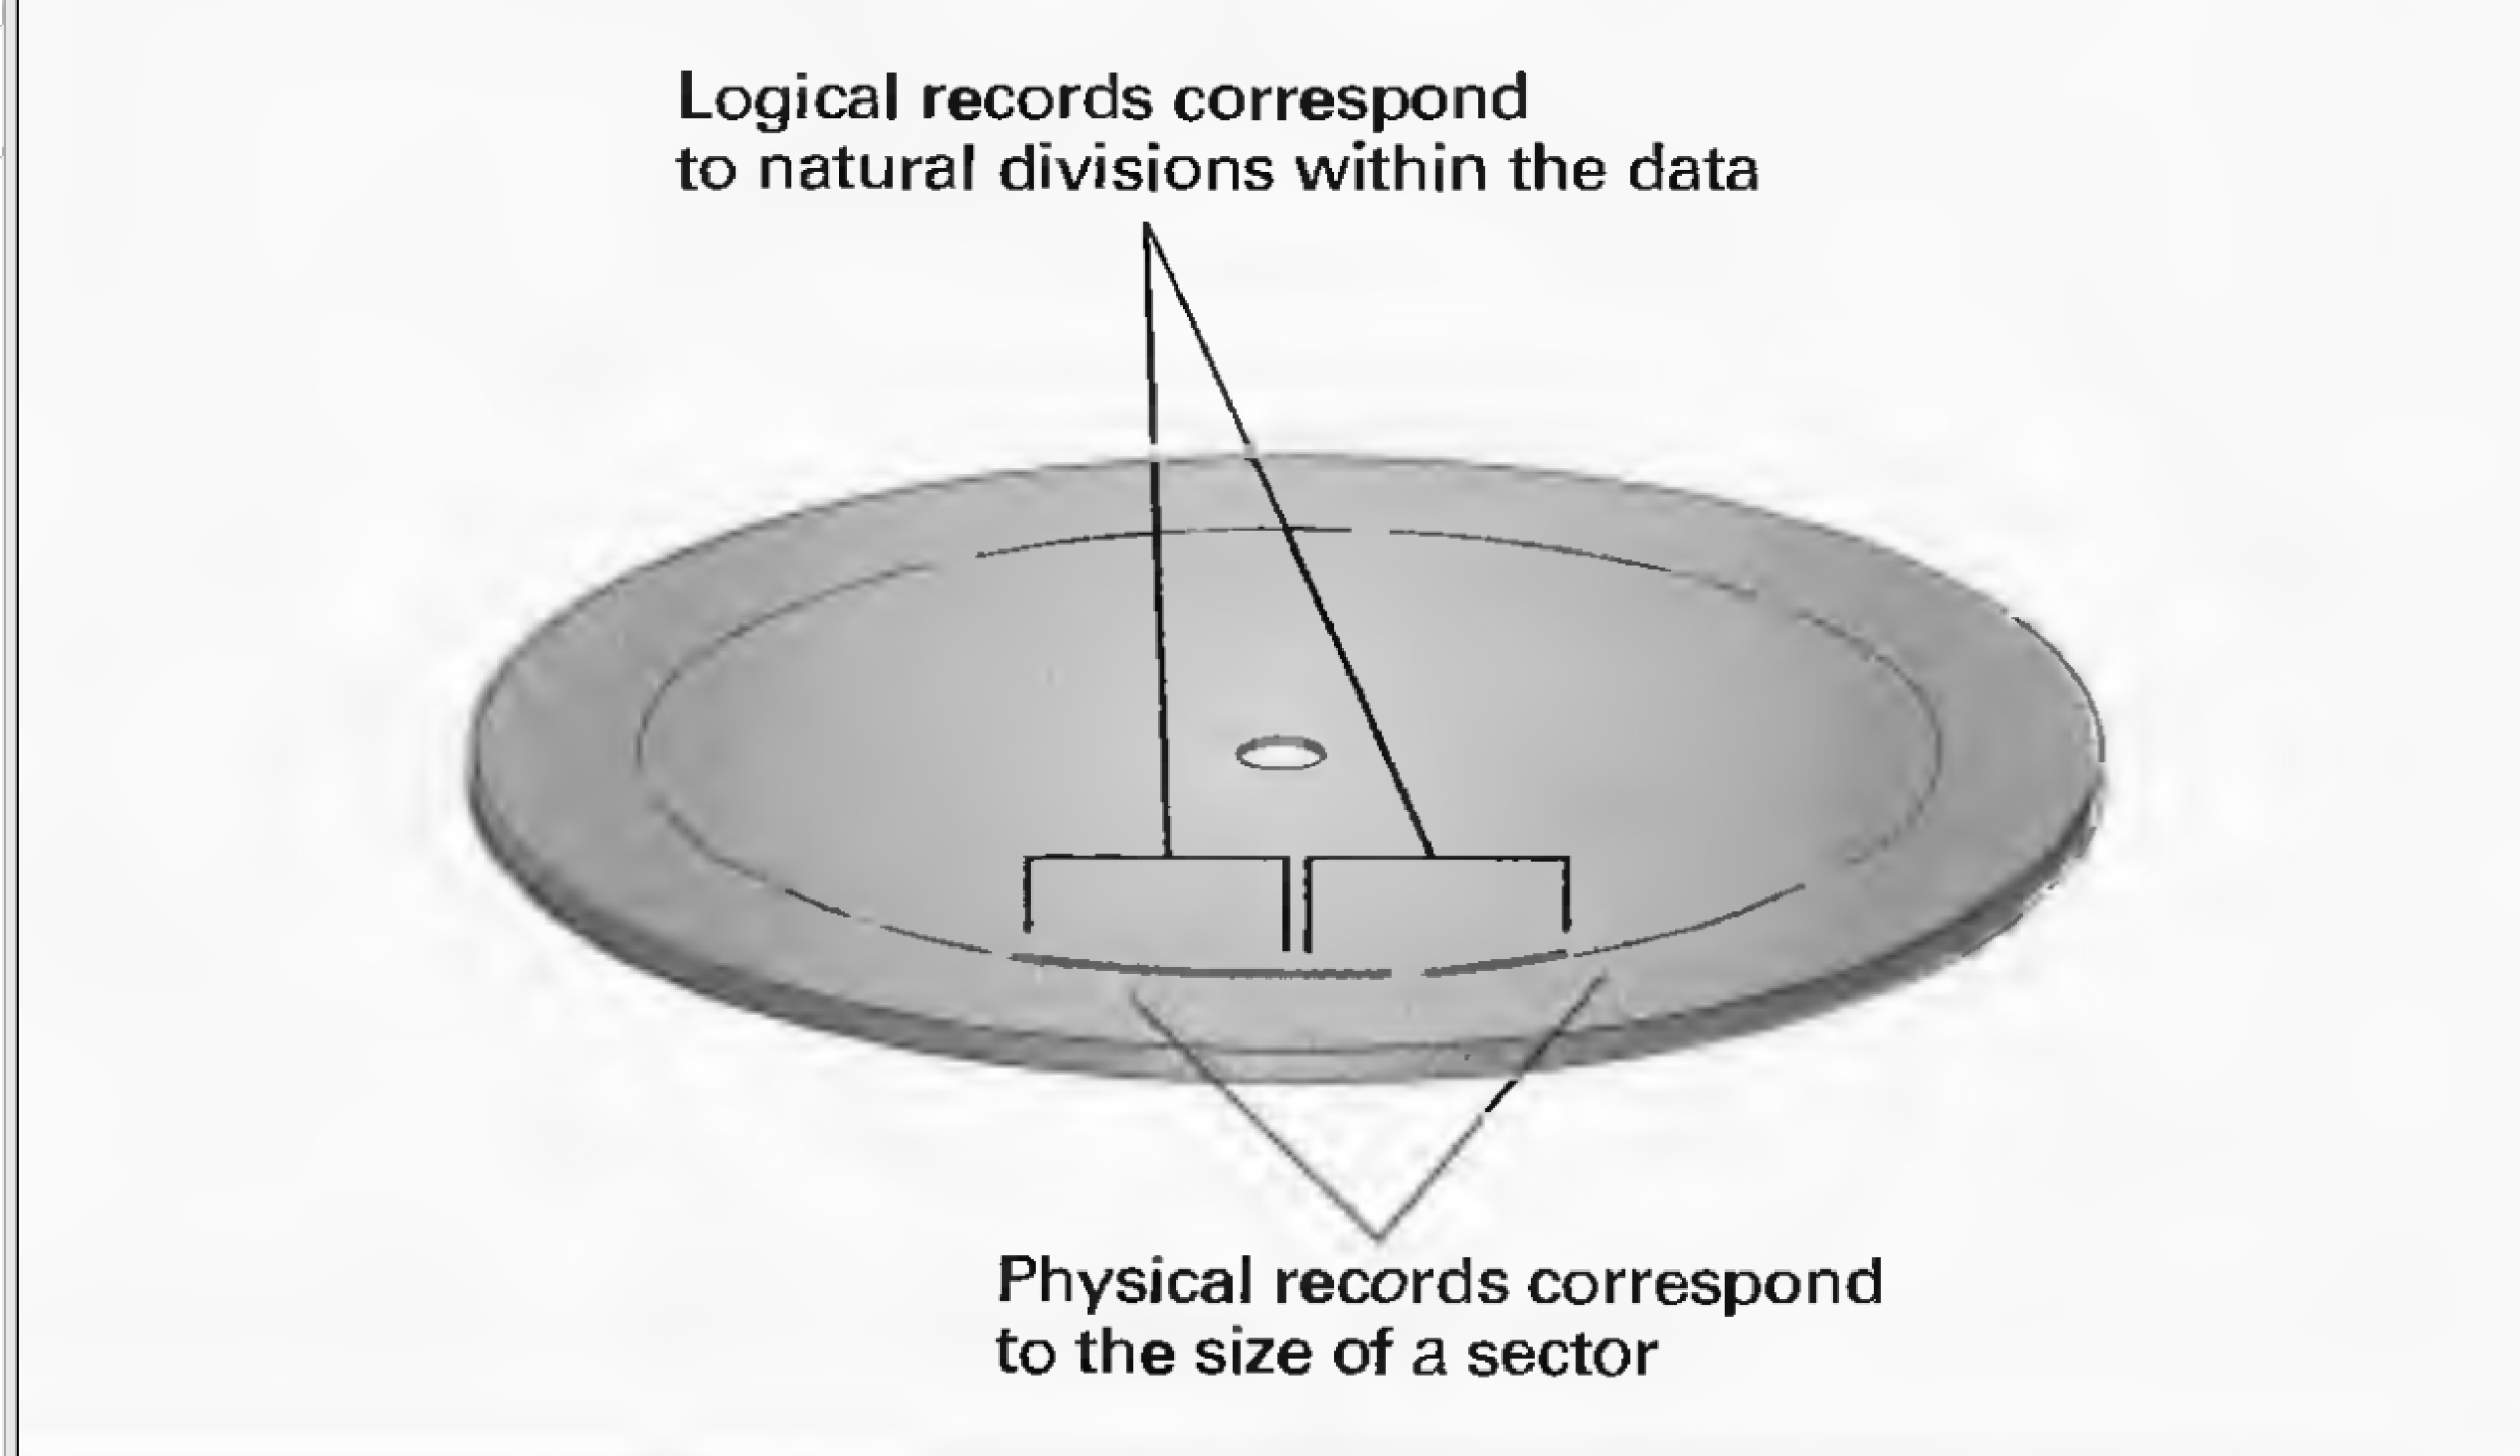
\includegraphics{ch2/Fig1-12.pdf}}
\caption{Bản ghi logic và bản ghi vật lý trên một đĩa}
  \label{fig:fig1.12}
\end{figure}

Các kích thước của bản ghi logic hiếm khi được so sánh với kích thước bản ghi vật lý của
của thiết bị lưu trữ khối. Nói cách khác, người ta có thể tìm thấy một vài bản ghi logic
nằm bên trong một bản ghi vật lý hoặc có thể là một bản ghi logic tách thành hai hoặc
nhiều bản ghi vật lý (Hình \ref{fig:fig1.12}). Kết quả là việc tìm kiếm dữ liệu từ thiết
bị lưu trữ khối phải kèm thêm với việc phục hồi những lộn xộn này. Một giải pháp chung cho
vấn đề này là đặt bên ngoài bộ nhớ chính khoảng đủ lớn lưu giữa một vài bản ghi vật lý và
để sử dụng không gian bộ nhớ này như một vùng nhóm lại. Có nghĩa rằng, các khối dữ liệu
thích hợp với bản ghi vật lý có thể được truyền giữa bộ nhớ chính và thiết bị lưu trữ
khối, trong khi dữ liệu nằm trong bộ nhớ chính có thể được tham khảo như bản ghi logic.


Một vùng bộ nhớ dùng theo cách này được gọi là \textbf{vùng đệm} (buffer). Nói chung, một
vùng đệm là một vùng nhớ được dùng để lưu trữ dữ liệu trung gian trong quá trình truyền dữ
liệu từ thiết bị này tới thiết bị khác. Ví dụ, các máy in hiện đại có chứa mạch nhớ riêng,
phần lớn của mạch này được dùng như vùng đệm để lưu trữ các phần của tài liệu còn chưa
được in mà máy in nhận được.
  
\subsection*{Câu hỏi \& Bài tập}

\begin{enumerate}
\item Hệ thống đĩa cứng có ưu điểm gì so với đĩa mềm khi các đĩa của nó quay nhanh hơn các
  đĩa của đĩa mềm?

\item Khi ghi dữ liệu trên hệ thống nhiều đĩa, ta nên hoàn thành hết bề mặt đĩa trước khi
  bắt đầu bề mặt khác, hay ta đầu tiên nên hoàn thành hết cylinder trước khi bắt đầu sang
  cylinder khác?

\item Trong một hệ thống đặt chỗ, dữ liệu thường phải cập nhật liên tục. Tại sao dữ liệu
  này nên được lưu trữ trên đĩa từ thay vì CD hay DVD?

\item Khi sửa một tài liệu với trình xử lý văn bản, đôi khi việc thêm đoạn văn bản không
  làm tăng kích thước bên ngoài của file trong lưu trữ khối. Nhưng có lúc chỉ thêm một kí
  tự cũng có thể làm tăng kích thước của file tới vài nghìn byte. Bạn hãy giải thích xem
  tại sao?

\item Nêu một vài ưu điểm của thiết bị flash so với hệ thống lưu trữ khác được giới thiệu
  trong phần này?


\item Vùng đệm là gì?
  
\end{enumerate}


  

%%% Local Variables: 
%%% mode: latex
%%% TeX-master: "../tindaicuong"
%%% End: 


\section{Biểu diễn thông tin}

Ta đã xem xét các kỹ thuật để lưu trữ các bít, bây giờ ta sẽ xem xét cách mã hoá thông tin
như dãy bít. Ta sẽ quan tâm đến các phương pháp phổ biến để mã hoá văn bản, dữ liệu số,
hình ảnh, âm thanh. [....]

\subsection*{Biểu diễn văn bản}
Thông tin của văn bản thường được biểu diễn bởi mã của các ký hiệu trong nó (như các chữ
cái trong một bảng chữ, các dấu chấm, phảy,...). Từ đó, văn bản được biểu diễn như một xâu
bít dài trong đó dãy bít liên tiếp biểu diễn các ký hiệu liên tiếp trong văn bản gốc.

Trong những năm~$1940$ và~$1950$, nhiều kiểu mã như vậy đã được thiết kế và được sử dụng
trong liên lạc giữa các thành phần khác nhau của thiết bị, điều này cũng dẫn đến phức tạp
trong truyền thông. Để làm giảm những phức tạp này, \textbf{Hội Chuẩn Quốc Gia Hoa Kỳ
  (ANSI)} đã chọn Mã chuẩn của Mỹ để trao đổi thông tin (\textbf{American Standard Code
  for Information Interchange (ASCII)}). Mã này dùng các xâu bảy bít để biểu diễn các chữ
cái hoa và chữ cái thường của bảng chữ Tiếng Anh, ký hiệu dấu, các số từ $0$ tới $9$, và
một số thông tin điều khiển như ký hiệu xuống dòng, ký hiệu trở về, và tab. Ngày nay, mã
ASCII được mở rộng sang thành dạng tám bít bằng cách thêm một $0$ vào bít trái nhất của
xâu bảy bít. Kỹ thuật này không chỉ cho ta một mã phù hợp với kích thước ô nhớ theo byte
mà còn cho ta thêm $128$ bít nữa (những mã bắt đầu bởi $1$) là những ký hiệu mở rộng thêm
từ bảng mã ASCII ban đầu. Không may, mỗi nhà sản xuất hướng sử dụng các ký hiệu được mở
rộng theo cách riêng của họ, nên dữ liệu mà các xâu bít này biểu diễn không dễ chuyển từ
các ứng dụng của nhà sản xuất này sang ứng dụng của nhà sản suất khác.

Một phần của ASCII theo định dạng xâu tám bít cho mỗi ký hiệu được chỉ ra bởi Phụ lục
\ref{}. Bằng cách tra phụ lục này, ta có thể giải mã xâu bít Hình~\ref{fig:fig1.13}
như thông điệp ``Hello.''.

\begin{figure}[bt]
\centering
\begin{tabular}{cccccc}
  $\underbrace{01001000}$ & $\underbrace{01100101}$
  & $\underbrace{01101100}$ & $\underbrace{01101100}$  
  & $\underbrace{01101111}$ & $\underbrace{00101110}$ \\
  \texttt{H}  & \texttt{e}  & \texttt{l} & \texttt{l} & \texttt{o}
  & \texttt{.}                                        \\
\end{tabular}
\caption{Thông điệp ``Hello.'' biểu diễn ở ASCII}
  \label{fig:fig1.13}
\end{figure}

Mặc dù bảng mã ASCII đã được thừa nhận rộng rãi trong nhiều năm, tuy nhiên do nhu cầu trình
bày tài liệu trong nhiều ngôn ngữ, những mã khác mở rộng hơn hiện nay lại trở nên phổ
biến. Một trong số đó là \textbf{Unicode}, đã được phát triển nhờ hợp tác của một vài nhà
sản xuất phần cứng hàng đầu và nhanh chóng nhận được sự ủng hộ của cộng đồng quốc tế. Mã
này dùng một xâu $16$ bít duy nhất để biểu biễn một ký hiệu. Vậy, Unicode bao gồm $65,536$
xâu bít khác nhau--đủ để biểu diễn các văn bản ở nhiều ngôn ngữ như Tiếng Trung, Tiếng
Nhật, và Tiếng Do Thái.

Chuẩn hoá cho một bộ mã đầy đủ Unicode được phát triển bởi \textbf{Tổ chức Quốc Tế về
  Chuẩn hoá} (International Organization for Standardization, viết tắt là
\textbf{ISO}). Mã này dùng các xâu độ dài $32$ bít, và có khả năng biểu diễn hàng tỉ ký
hiệu khác nhau.

Một file bao gồm một dãy ký hiệu dài được mã hoá dùng ASCII hoặc Unicode thường được gọi
là một \textbf{file văn bản}. Một ý quan trọng mà ta phải phân biệt, đó là giữa một file
văn bản đơn giản có thể thao tác bởi các chương trình công cụ được gọi là \textbf{trình
  soạn thảo} và các file phức tạp hơn được tạo bởi \textbf{bộ xử lý văn bản}. Cả hai đều
bao gồm các văn bản. Tuy nhiên, một file văn bản chỉ chứa các ký hiệu mã hoá của văn bản,
trong khi đó một file tạo bởi bộ xử lý văn bản chứa nhiều mã riêng biểu diễn các font, các
thông tin về cách gióng hàng,... Hơn nữa, bộ xử lý văn bản có thể sử dụng các mã riêng
thay vì chuẩn ASCII hoặc Unicode để biểu diễn văn bản.

\subsection*{Biểu diễn giá trị số}

Lưu trữ thông tin theo cách mã hoá các ký tự là không hiệu quả khi thông tin là các giá
trị số. Để thấy lý do tại sao, ta cùng xem xét vấn đề lưu trữ giá trị $25$. Nếu ta nhất
định lưu trữ nó như các ký hiệu ở dạng ASCII dùng mỗi byte cho mỗi ký hiệu, ta cần $16$
bít để lưu trữ. Hơn nữa, số lớn nhất ta có thể lưu trữ dùng $16$ bít là $99$. Tuy nhiên,
nếu dùng \textbf{ký hiệu nhị phân} thì với $16$ bít ta có thể lưu trữ mọi số nguyên từ $0$
tới $65,535$. Bởi vậy, ký hiệu nhị phân (hay các dạng khác của nó) được sử dụng rộng rãi
cho việc mã hoá dữ liệu số trên máy tính.

Ký hiệu nhị phân là một cách biểu diễn các giá trị số chỉ dùng các số $0$ và $1$ thay vì
các số $0, 1, 2 , 3, 4, 5, 6, 7, 8, $ và $9$ như trong chữ số truyền thống, hoặc cơ sở
$10$. ta sẽ nghiên cứu hệ thống số đầy đủ trong Mục \ref{}. Bây giờ, ta sẽ chỉ cần một vài
kiến thức cơ sở để hiểu hệ thống này. Với mục đích này, ta sẽ xem xét đồng hồ đo số km
trong các ôtô kiểu cũ [.....]

Do tính hiệu quả này, các thông tin dạng số thường được lưu trữ bởi một dạng ký hiệu nhị
phân thay vì dạng ký hiệu được mã hoá. Ta nói ``một dạng ký hiệu nhị phân'' bởi vì hệ
thống nhị phân được mô tả trực tiếp chỉ là cơ sở cho một vài kỹ thuật lưu trữ số được sử
dụng bên trong máy. Một vài dạng khác của hệ thống nhị phân sẽ được thảo luận sau này. Bây
giờ, ta thuần tuý chỉ để ý rằng hệ thống được gọi là ký hiệu \textbf{bù hai} (xem Phần
\ref{}) là cách chung để lưu trữ các số bởi vì nó cho ta phương pháp thích hợp để biểu
diễn số ấm cũng như số nguyên dương. Để biểu diễn phân số như $4\frac{1}{2}$ hoặc
$\frac{3}{4}$, được gọi là ký hiệu \textbf{dấu chấm động} (xem Mục \ref{}).

\subsection*{Biểu diễn hình ảnh}

Các ứng dụng máy tính ngày nay bao gồm nhiều hơn là chỉ có văn bản và giá trị số. Chúng
còn bao gồm cả hình ảnh, âm thanh, và video. Kỹ thuật phổ biến để biểu diễn ảnh bao gồm
hai loại: \textbf{các kỹ thuật bitmap} và \textbf{các kỹ thuật vectors}. Với kỹ thuật bit
map, một ảnh được biểu diễn như một tập các điểm, mỗi điểm gọi là một \textbf{pixel}, viết
tắt của từ ``picture element.'' (phần tử ảnh). Một ảnh đen trắng được mã hoá như một xâu
bít dài biểu diễn các dòng pixel trong ảnh, trong đó mỗi bít hoặc là bằng $1$ hoặc
bằng~$0$ phụ thuộc khi nào pixel tương ứng là đen hay trắng. Kỹ thuật này được sử dụng
trong hầu hết các máy sao chép (facsimile).

Thuật ngữ \textit{bit map} bắt nguồn từ sự kiện rằng các bít biểu diễn một ảnh theo định
dạng một-bít-cho-một-pixel [...]. Ngày nay thuật ngữ đã được tổng quát hoá để bao gồm mọi
hệ thống trong đó các ảnh được mã hoá theo cách pixel-cạnh-pixel. Ví dụ, trong trường hợp
ảnh đen trắng, mỗi pixel được biểu diễn bởi một tập các bít (thường là tám), cho phép bóng
xám được biểu diễn.

Cách tiếp cận bip map được mở rộng cho ảnh màu, trong đó mỗi điểm ảnh (pixel) được biểu
diễn bởi một tổ hợp các bít chỉ ra có mặt của pixel. Hai cách tiếp cận này là chung. Trong
đó, cách ta sẽ gọi là mã hoá RGB, mỗi điểm ảnh được biểu diễn bởi thành phần màu-- đỏ
(red), xanh lá cây (green) và xanh lam (blue)--tương ứng với ba màu của ánh sáng. Thông
thường ta dùng một byte để biểu diễn cường độ của mỗi thành phần màu. Bởi vậy, mỗi điểm
ảnh cần ba byte để lưu trữ.

Một lựa chọn phổ biến khác để mã hoá RGB là sử dụng thành phần ``độ sáng'' kết hợp với hai
thành phần màu. Ở đây, thành phần ``độ sáng'' được gọi là độ chiếu sáng của điểm ảnh, về
cơ bản nó là tổng của ba thành phần đỏ, xanh lá cây và xanh lam. (Trên thực tế, nó chính
là tổng số ánh sáng trắng trong điểm ảnh, nhưng ở đây ta sẽ không cần quan tâm chi tiết.)
Hai thành phần còn lại được gọi là độ màu xanh lam và độ màu đỏ. Độ màu xanh lam (tương
ứng, độ màu đỏ) được xác định bằng cách tính chênh lệch giữa độ chiếu sáng của điểm ảnh và
tổng số ánh sáng xanh lam (tương ứng tổng số ánh sáng đỏ) trong điểm ảnh. Kết hợp cả ba
thành phần này lại ta được thông tin xác định điểm ảnh.

Tính phổ biến của mã hoá ảnh dùng độ sáng và các thành phần màu bắt nguồn từ lĩnh vực
truyền hình màu bởi vì cách tiếp cận này cho phép tương thích giữa việc mã hoá các ảnh màu
và các tín hiệu nhận được của các tivi đen trắng đời cũ. Thực ra, các ảnh xám có thể được
xem như ảnh màu khi giới hạn chỉ dùng thành phần độ sáng.

Một điểm bất lợi của kỹ thuật bitmap là ảnh không thể thay đổi kích thước một cách tuỳ
ý. Về cơ bản, chỉ có cách phóng to ảnh là tăng độ lớn của điểm ảnh, nhưng nó sẽ làm vỡ
ảnh. (Đây là kỹ thuật dùng trong các camera số gọi là ``digital zoom'', ngược lại với
``optical zoom'' là điều chỉnh thấu kính của cameras.) Kỹ thuật vector cho phép khắc phục
vấn đề này. Với cách tiếp cận này, một ảnh được biểu diễn như một tập các đường thẳng và
đường cong. Kiểu mô tả này bỏ qua chi tiết xem làm thế nào các đường thẳng và đường cong
được vẽ ra thiết bị tạo ảnh mà thay vào đó nó nhấn mạnh đến cách tạo ra một mẫu điểm ảnh
đặc biệt.

Nhiều font trong các hệ thống xử lý văn bản ngày nay được mã hoá dùng kỹ thuật vector. Kỹ
thuật này cho phép làm thay đổi kích thước của ký tự trong văn bản một cách mềm dẻo. Các
font này được gọi là \textbf{scalable fonts}. Ví dụ, TrueType (được phát triển bởi
Microsoft và Apple Computer) là một hệ thống mô tả cách các ký hiệu trong văn bản được
vẽ. Tương tự, PostScript (được phát triển bởi Adobe System) cho phép mô tả các ký tự cũng
như các dữ liệu ảnh tổng quát hơn. Các kỹ thuật biểu diễn vector cũng phổ biến trong các
hệ thống \textbf{thiết kế với trợ giúp của máy tính} (Computer-aided design) trong đó việc
vẽ các đối tượng ba chiều được hiện và được thao tác trên màn hình máy tính.

\subsection*{Biểu diễn âm thanh}

Phương pháp chung nhất để mã hoá thông tin audio để lưu trữ và xử lý trong máy tính là lấy
mẫu biên độ của sóng âm theo từng khoảng và ghi lại như dãy giá trị. Ví dụ, dãy $0$,
$1.5$, $2.0$, $3.0$, $4.0$, $3.0$, $0$ là dãy sóng âm theo biên độ, nói một cách ngắn gọn,
sóng này tăng dần rồi quay lại $0$ (Hình \ref{fig:fig1.14}). Kỹ thuật này sử dụng một tỷ lệ lấy mẫu
là $8000$ mẫu mỗi giây, đã được dùng trong nhiều năm để truyền thông điện thoại khoảng
cách xa. Giọng nói được mã hoá bằng giá trị số biểu diễn biên độ của giọng $8000$ lần
trong một giây. Các giá trị này được truyền đến nơi nhận, tại đây âm của giọng được tái
tạo lại.


Dù tỷ lệ $8000$ mẫu trên giây có vẻ khá nhanh, nhưng nó vẫn không đủ để thu âm với độ
trung thực cao. Để đạt được chất lượng âm thanh cao của đĩa CD nhạc, một tỷ lệ mẫu
$44,100$ mẫu trên giây được dùng. Dữ liệu đạt được từ mỗi mẫu được biểu diễn bởi $16$ bít
($32$ bít cho thu âm stereo). Vậy nên ta cần hơn một triệu bít cho mỗi giây của âm nhạc
thu ở dạng stereo.

\begin{figure}[tbh]
\centering
    \scalebox{0.65}{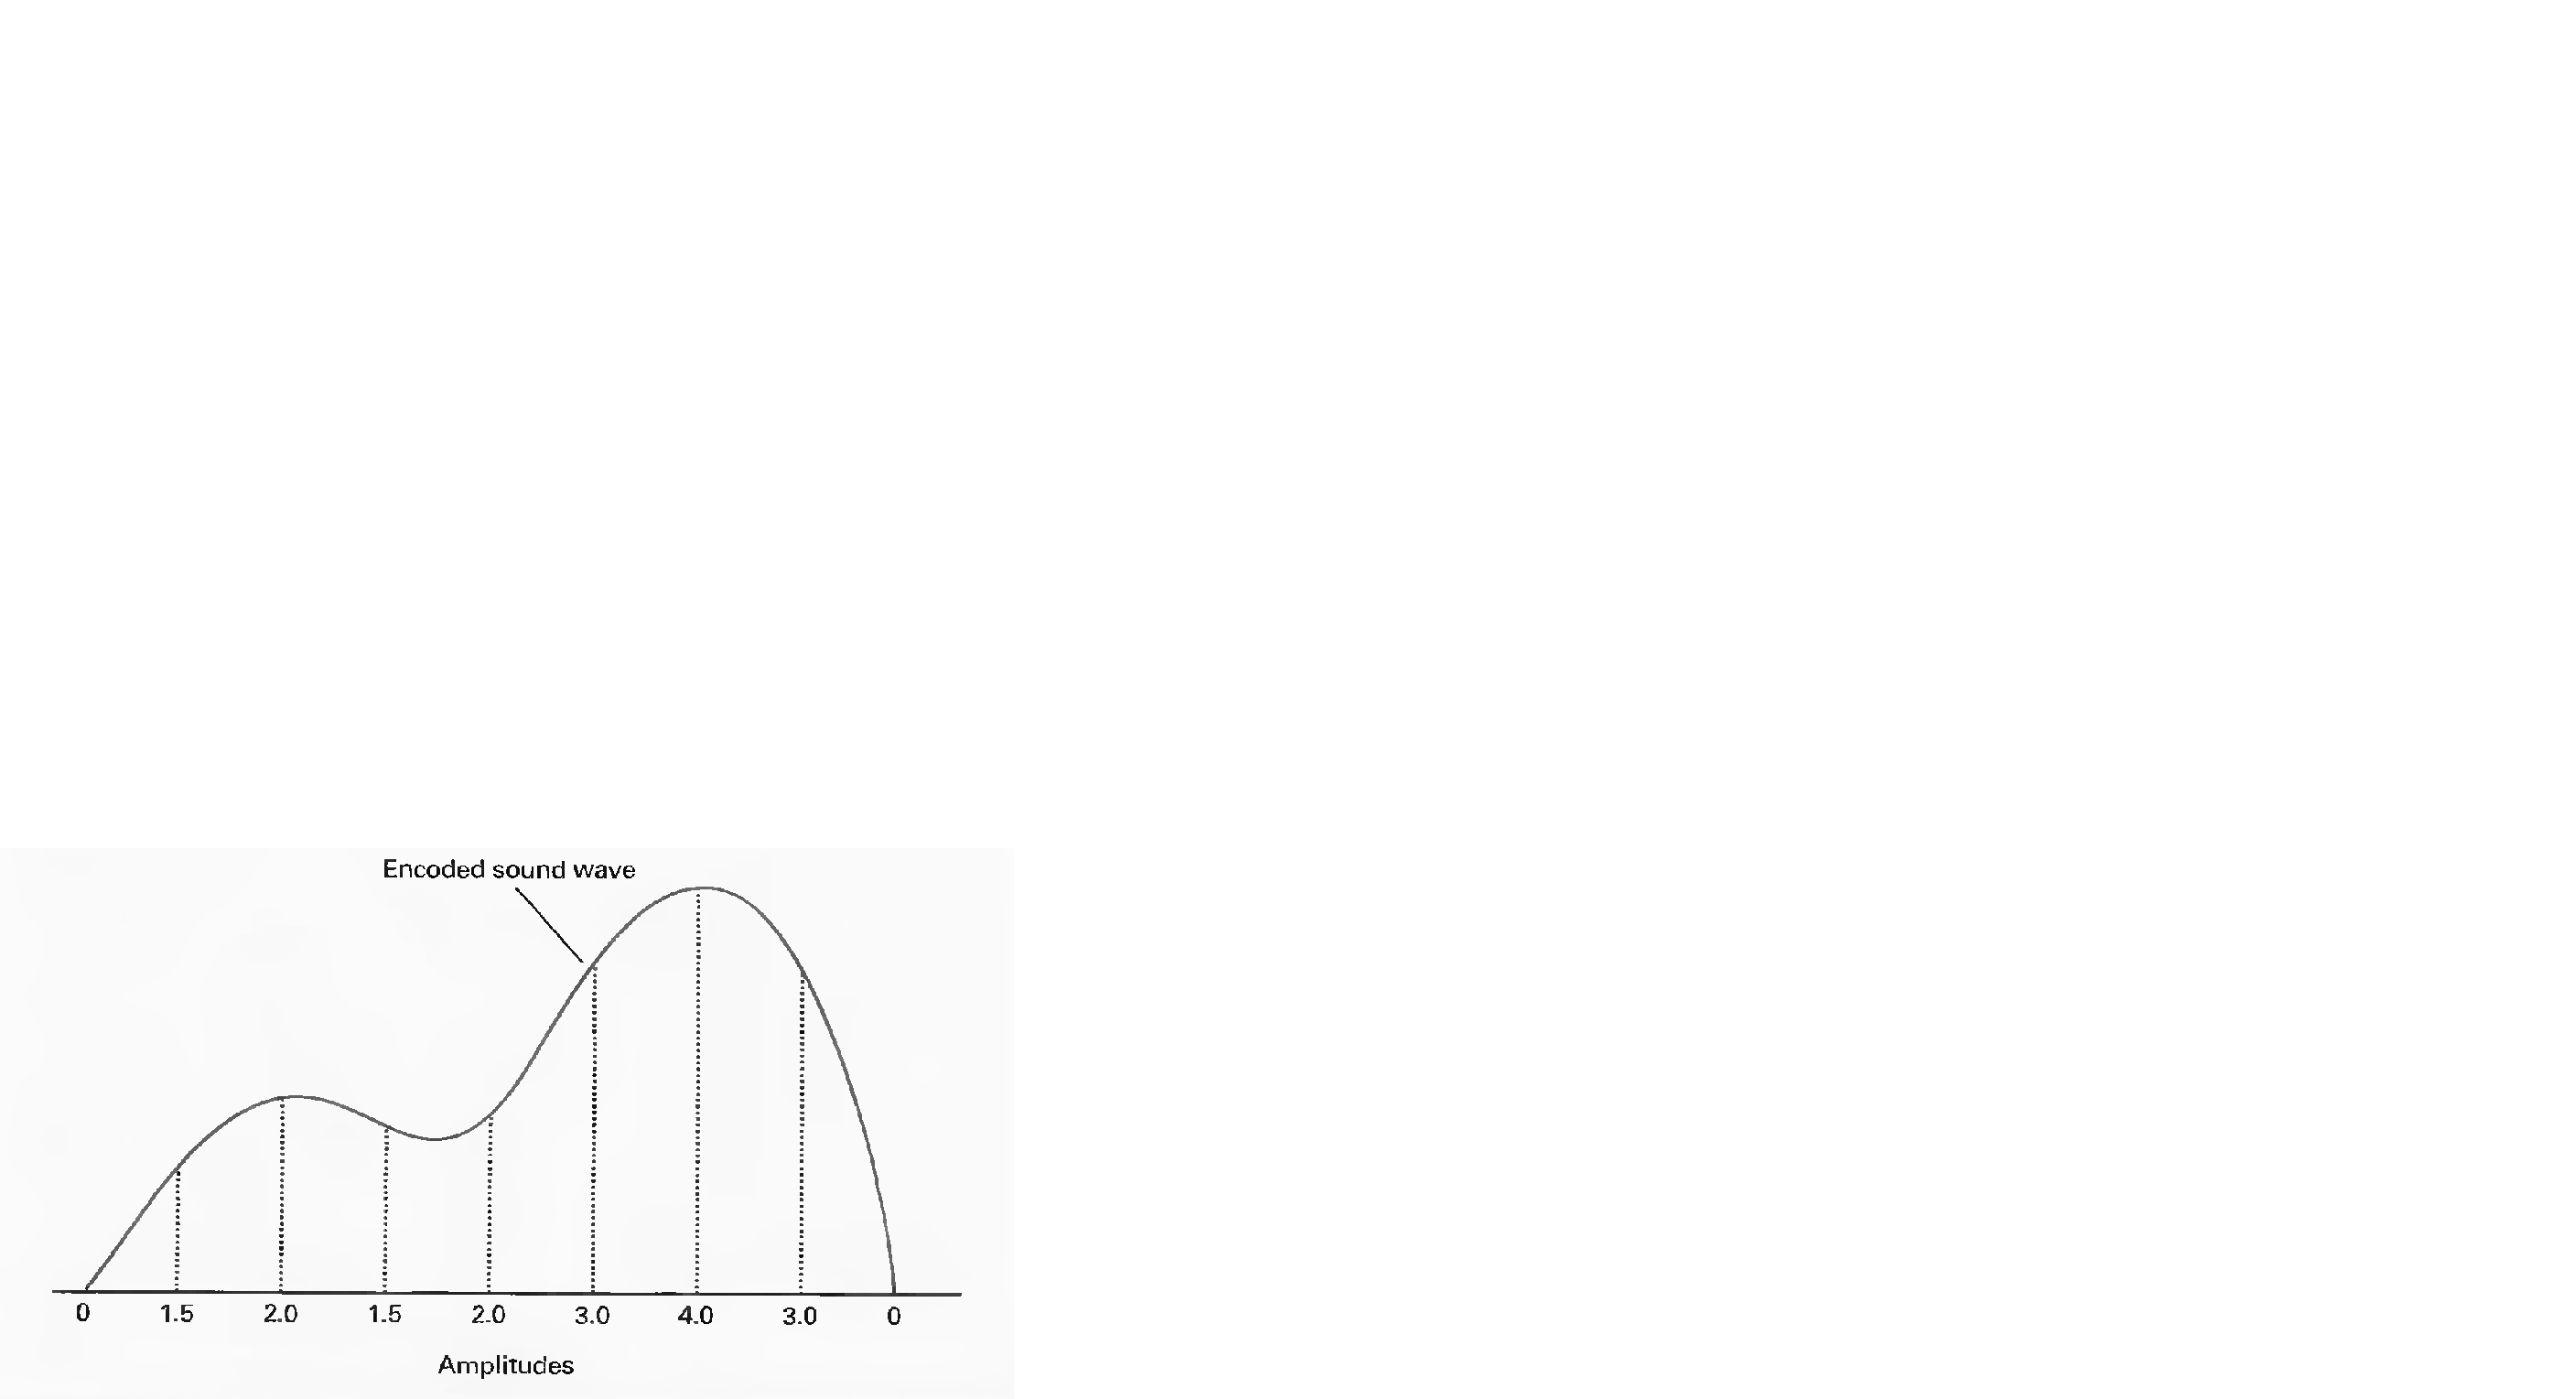
\includegraphics{ch2/Fig114.pdf}}
    \caption{Sóng âm được biểu diễn bởi dãy $0$, $1.5$, $2.0$, $3.0$, $4.0$, $3.0$, $0$}
  \label{fig:fig1.14}
\end{figure}


Một hệ thống mã hoá khác là Musical Instrumental Digital Interface (MIDI) được sử dụng
rộng rãi được sử dụng trong các bộ tổng hợp được tìm thấy trong các bàn phím điện tử,
trong âm thanh của các trò chơi video, và trong âm thanh hiệu ứng kèm các các trang
web. Bằng cách mã hoá các chỉ dẫn để tạo ra âm cho một thiết bị tổng hợp thay vì phải mã
hoá bản thân âm thanh, MIDI tránh được các yêu cầu lưu trữ lớn của kỹ thuật lấy mẫu. Chính
xác hơn, MIDI mã hoá các nốt nhạc của các nhạc cụ theo thời gian, ví dụ clarinet chơi nốt
Rê trong hai giây có thể mã hoá bằng ba byte thay vì mất hơn hai triệu bít bằng cách lấy
mẫu với tỷ lệ $44,100$ mẫu trên giây.

Nói tóm lại, ta có thể nghĩ MIDI như cách mã hoá các bản nhạc đọc bởi người biểu diễn thay
vì chính bản thân việc trình diễn, và việc chơi một file MIDI có thể nghe rất khác trên
các thiết bị tổng hợp khác nhau.

\subsection*{Câu hỏi \& Bài tập}

\begin{enumerate}
\item Đây là một thông điệp được mã hoá ở dạng ASCII dùng tám bít cho mỗi ký hiệu. Thông
  điệp này ý nghĩa là gì? (Xem Phụ lục \ref{})

\begin{tabular}{cccccc}
  01000011 &01101111 &01101101 &01110000 &01110101 &01110100  \\
  01100101 &01110010 &00100000 &01010011 &01100011 &01101001  \\
  01100101 &01101110 &01100011 &01100101 & &
\end{tabular}


\item Hãy chỉ ra mối quan hệ giữa mã của ký tự hoa và ký tự thường của
  cùng một ký tự theo bảng mã ASCII.

\item Mã hoá các câu sau theo bảng mã ASCII.
  \begin{enumerate}
  \item Where are you?

  \item "How?" Cheryl asked.

  \item 2 + 3 = 5.
  \end{enumerate}

\item Hãy mô tả một thiết bị trong cuộc sống hàng ngày có thể ở một trong hai trạng thái,
  ví dụ như lá cờ cắm trên cột cờ có thể ở trạng thái được treo hay không treo. Gán ký
  hiệu $1$ tới một trong hai trạng thái này và $0$ cho trạng thái còn lại, và chỉ ra cách
  biểu diễn ASCII cho ký tự $b$ khi lưu trữ dùng kiểu bít này.

\item Chuyển mỗi biểu diễn nhị phân sau đây sang cơ số mười:

  \begin{inparaenum}
  \item $0101 $ \hspace{2cm}
  \item $1001 $ \hspace{2cm}
  \item $1011 $

  \item $0110 $ \hspace{2cm}
  \item $10000$ \hspace{2cm}
  \item $10010$
  \end{inparaenum}

\item Chuyển mỗi biểu diễn thập phân sau đây sang nhị phân:

  \begin{inparaenum}
  \item $6$ \hspace{2cm} 
  \item $13$ \hspace{2cm}
  \item $11$ \hspace{2cm}


  \item $18$ \hspace{2cm}
  \item $27$ \hspace{2cm}
  \item $4$
  \end{inparaenum}

\item Nếu mỗi chữ số được mã hoá bởi một byte theo ASCII thì giá trị số lớn nhất có thể
  được biểu diễn dùng ba bytes là bao nhiêu? cũng vẫn ba byte đó nếu ta dùng ký hiệu nhị
  phân thì giá trị số lớn nhất là bao nhiêu?

\item Một lựa chọn khác so với ký hiệu hexa để biểu diễn dãy bít là \textbf{ký hiệu thập
    phân ngăn cách bởi dấu chấm} trong đó mỗi byte biểu diễn bởi giá trị ở cơ sở $10$
  tương đương. byte biểu diễn một số ngăn cách bởi các dấu chấm. Ví dụ, $12.5$ biểu diễn
  xâu $0000110000000101$ (byte $00001100$ biểu diễn số $12$, và $00000101$ biểu diễn số
  $5$), và xâu $100010000001000000000111$ được biểu diễn số $136.16.7$. Hãy biểu diễn mỗi
  xâu bít sau đây theo ký hiệu thập phân ngăn cách bởi dấu chấm.

  \begin{inparaenum}[a.]
  \item $0000111100001111$ \hspace {3cm}
  \item $001100110000000010000000$

  \item $0000101010100000$
  \end{inparaenum}

\item Chỉ ra ưu điểm của cách biểu diễn ảnh dùng kỹ thuật vector so với các kỹ thuật
  bitmap? ưu điểm của kỹ thuật bipmap so với kỹ thuật vector?

\item Giả sử ta dùng kỹ thuật lấy mẫu với $44,100$ mẫu trong một giây để thu âm stereo một
  giờ âm nhạc giống như đã thảo luận ở trên. Hãy so sánh kích thước của phiên bản được mã
  hoá theo cách này với một đĩa CD.
\end{enumerate}


















%%% Local Variables: 
%%% mode: latex
%%% TeX-master: "../tindaicuong"
%%% End: 


\section{Bài tập cuối chương}
\begin{multicols}{2}
  \begin{enumerate}

  \item Hãy xác định đầu ra của mỗi mạch sau đây, giả sử đầu vào phía trên là $1$ và đầu
    vào phía dưới là $0$.
    \begin{enumerate}
    \item \scalebox{0.6}{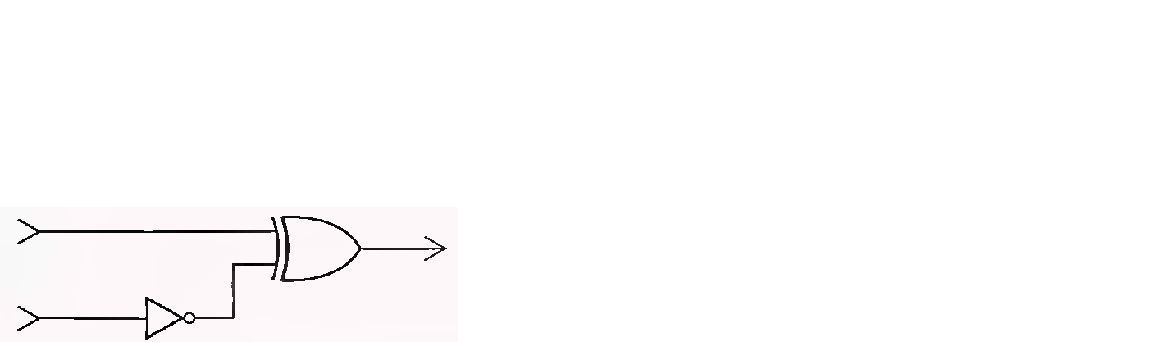
\includegraphics{ch2/ex21a.pdf}}

    \item \scalebox{0.6}{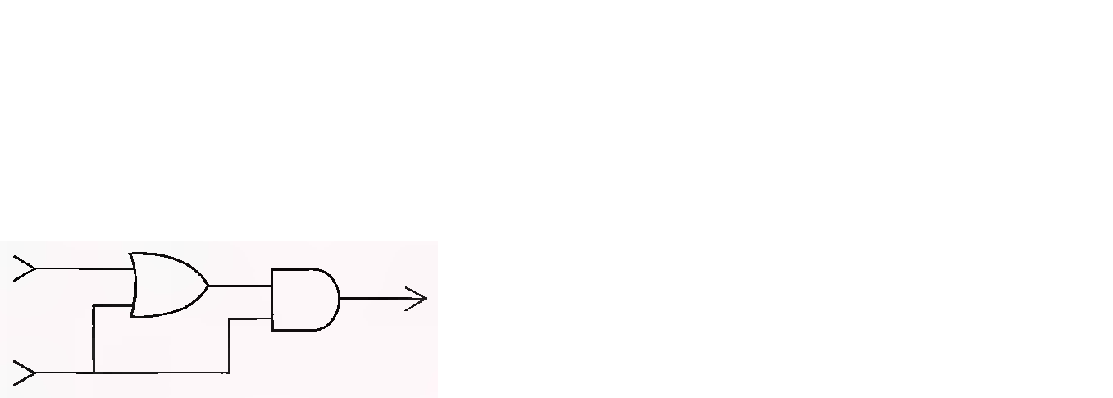
\includegraphics{ch2/ex21b.pdf}}

    \item \scalebox{0.6}{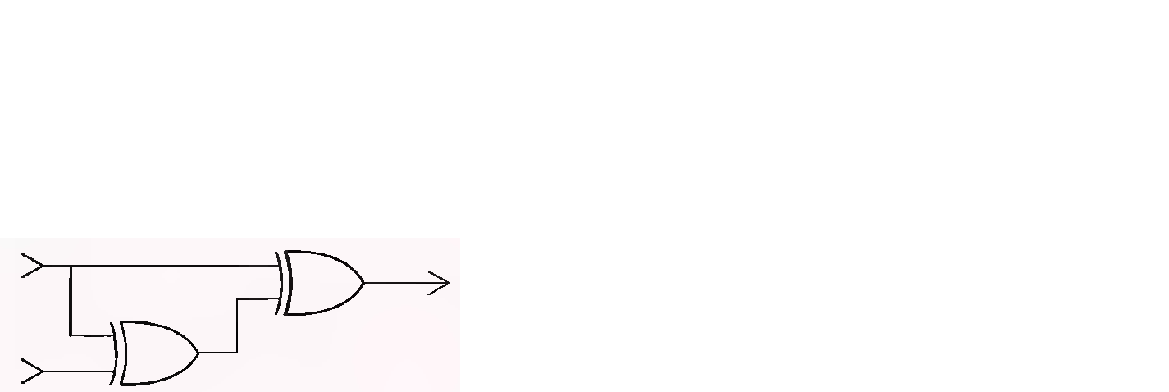
\includegraphics{ch2/ex21c.pdf}}
    \end{enumerate}
  \item Với mỗi mạch dưới đây, hãy xác định các tổ hợp đầu vào để đầu ra là $1$.
    \begin{enumerate}
    \item \scalebox{0.6}{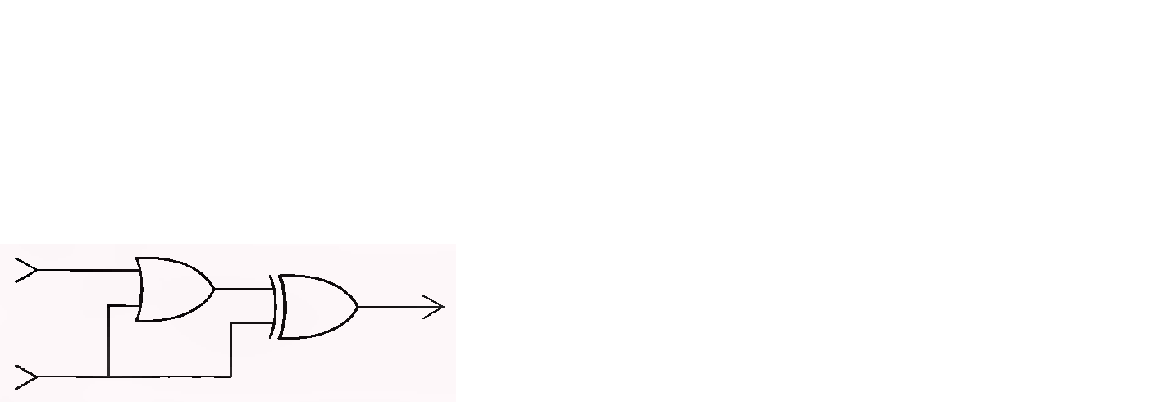
\includegraphics{ch2/ex22a.pdf}}

    \item \scalebox{0.6}{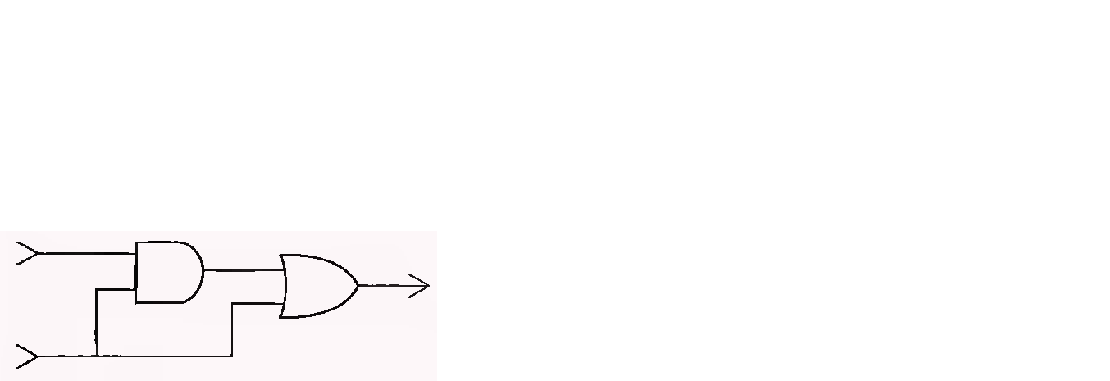
\includegraphics{ch2/ex22b.pdf}}

    \item \scalebox{0.6}{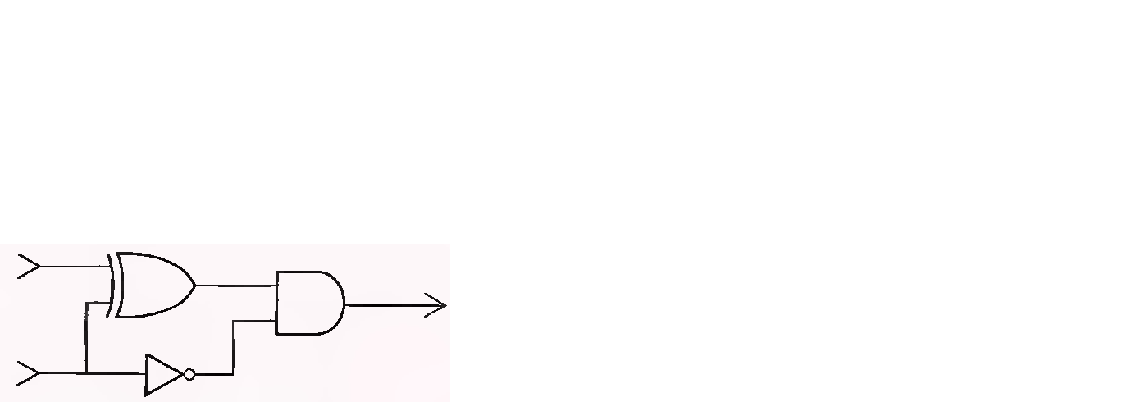
\includegraphics{ch2/ex22c.pdf}}

    \end{enumerate}

  \item Trong mỗi mạch dưới đây, các hình chữ nhật biểu diễn cùng một loại cổng. Dựa vào
    thông tin đầu vào và đầu ra, hãy xác định cổng liên quan trong hình là $\AND$, $\OR$
    hay $\XOR$.
    \begin{enumerate}
    \item \scalebox{0.6}{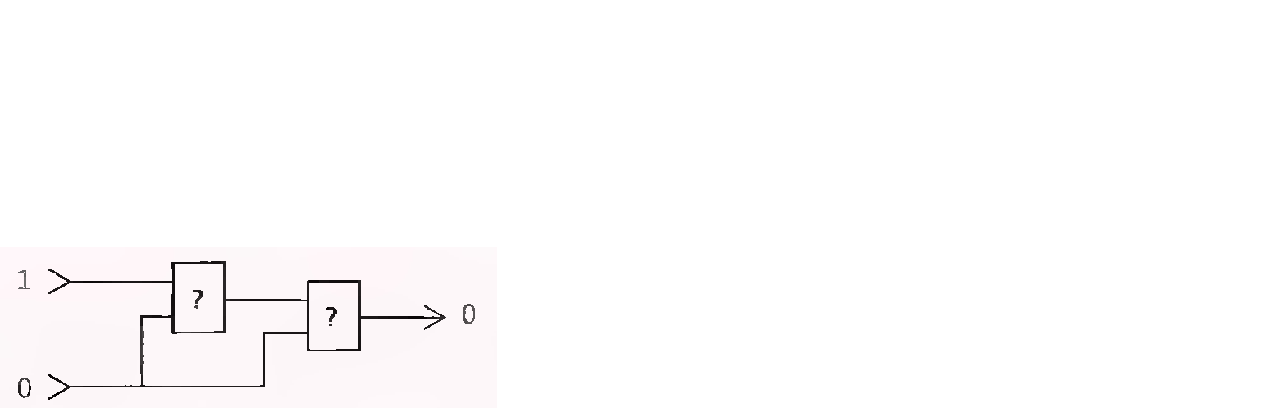
\includegraphics{ch2/ex23a.pdf}}

    \item \scalebox{0.6}{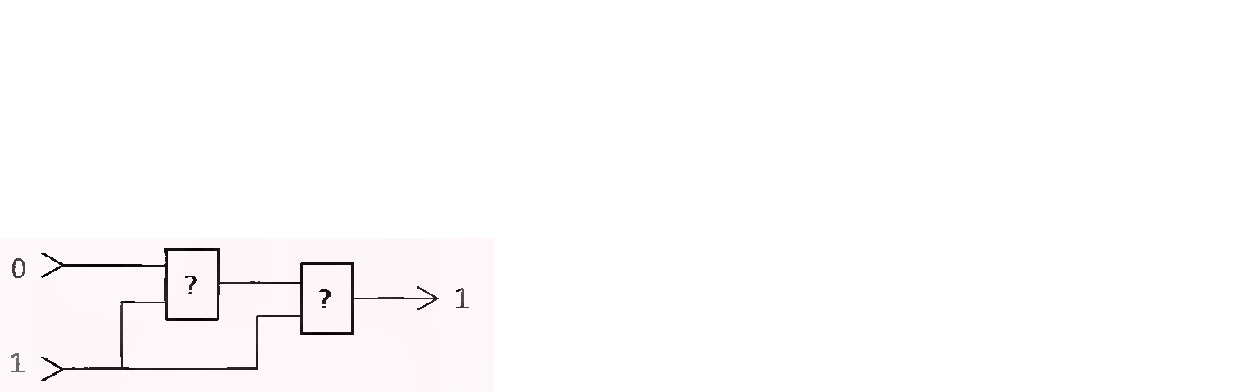
\includegraphics{ch2/ex23b.pdf}}

    \item \scalebox{0.6}{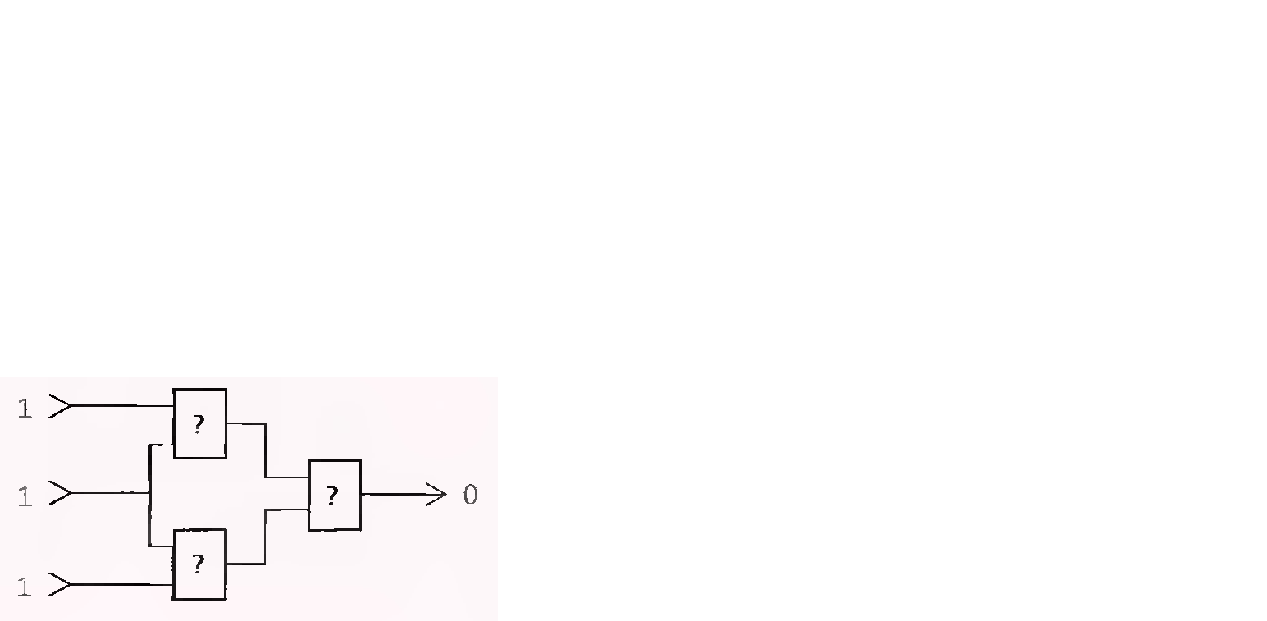
\includegraphics{ch2/ex23c.pdf}}

    \end{enumerate}

  \item Giả sử rằng cả đầu vào và đầu ra trong mạch dưới đây là $1$. Mô tả xem chuyện gì
    xảy ra nếu đầu vào phía trên tạm thời thay đổi về $0$. Mô tả xem chuyện gì xảy ra nếu
    đầu vào phía dưới tạm thời thay đổi về $0$. Vẽ lại mạch sử dụng các cổng $\NAND$.
    \begin{center}
      \scalebox{0.7}{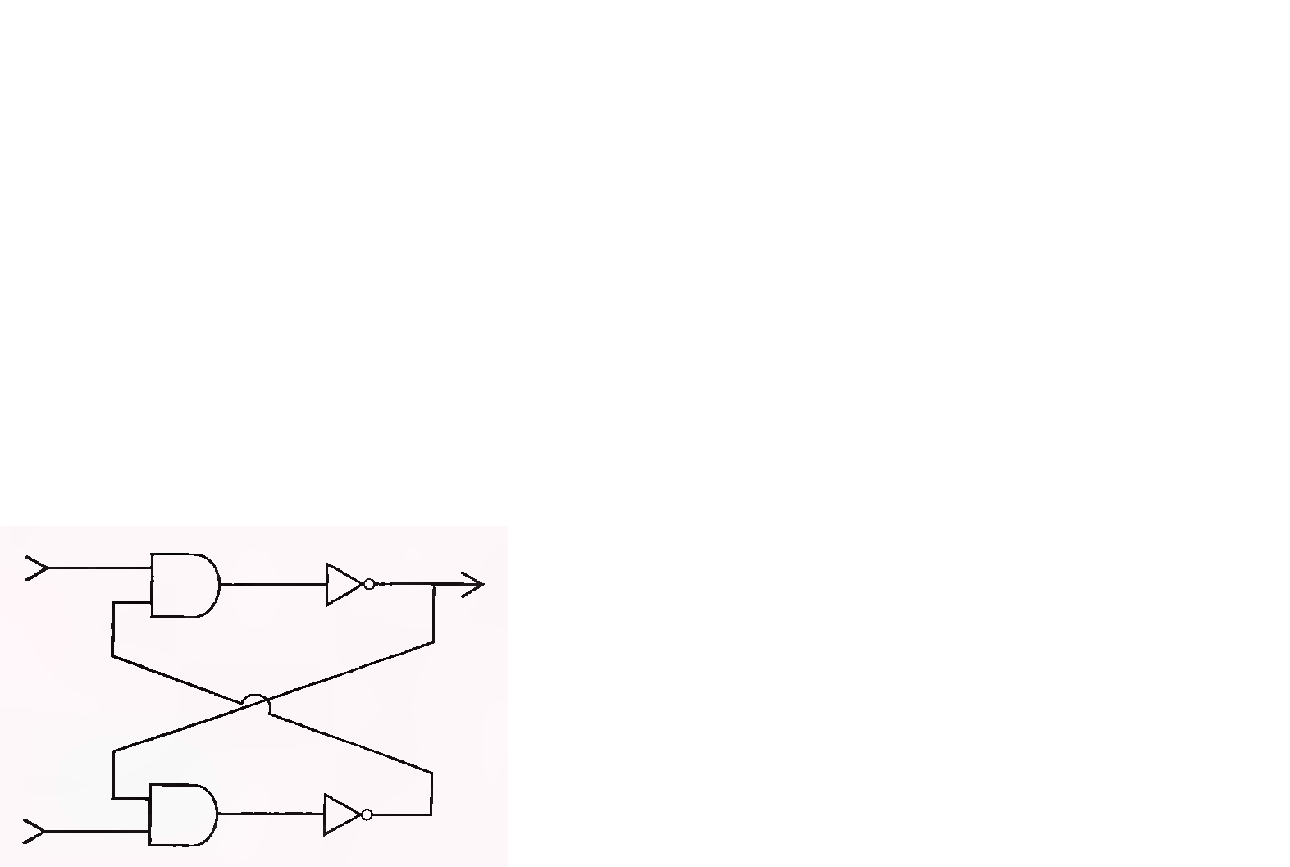
\includegraphics{ch2/ex24.pdf}}
    \end{center}
  \item Bảng dưới đây biểu diễn địa chỉ và nội dung (dùng ký hiệu hexa) của một vài ô nhớ
    trong bộ nhớ chính của máy tính. Hãy thực hiện theo dãy các lệnh ở dưới đây và ghi lại
    nội dung của các ô nhớ này.

    \begin{tabular}[c]{cc}
      Địa chỉ & Nội dung \\
      $00$ & $AB$ \\
      $01$ & $53$ \\
      $02$ & $D6$ \\
      $03$ & $02$
    \end{tabular}
    \begin{enumerate}[B1. ]
    \item Chuyển nội dung của ô nhớ có địa chỉ là $03$ vào ô nhớ địa chỉ~$00$.

    \item Chuyển giá trị $01$ vào ô nhớ tại địa chỉ $00$.

    \item Chuyển giá trị được lưu trữ tại địa chỉ $01$ vào ô nhớ tại địa chỉ~$03$.
    \end{enumerate}

  \item Nếu địa chỉ mỗi ô nhớ của một máy được biểu diễn bởi hai số hexa, vậy có bao nhiêu
    ô nhớ trong bộ nhớ chính của máy tính này?  có bao nhiêu ô nhớ nếu mỗi ô nhớ biểu diễn
    bởi bốn số hexa?

  \item Xâu bít gì được biểu diễn bởi ký hiệu hexa sau đây?

    \begin{inparaenum}[a.]
    \item $CB$ \quad
    \item $67$ \quad
    \item $A9$ \quad
    \item $10$ \quad
    \item $FF$
    \end{inparaenum}

  \item Giá trị của bít trọng số cao nhất trong xâu bít được biểu diễn bởi các ký hiệu
    hexa sau đây là gì?

    \begin{inparaenum}[a.]
    \item $7F$ \quad
    \item $FF$ \quad
    \item $8F$ \quad
    \item $1F$
    \end{inparaenum}

  \item Biểu diễn các xâu bít dưới đây thành ký hiệu hexa:
    \begin{enumerate}[a.]
    \item $101010101010$
    \item $110010110111$
    \item $000011101011$
    \end{enumerate}

  \item Giả sử một camera số có một khả năng lưu trữ là $256$MB. Có bao nhiêu bức ảnh có
    thể được lưu trữ trong camera nếu mỗi ảnh bao gồm $1024$ điểm ảnh trên một dòng và
    $1024$ điểm ảnh trên một cột và nếu mỗi điểm ảnh cần ba byte để lưu trữ.

  \item Giả sử một bức ảnh được biểu diễn trên màn hình máy tính bởi một mảng hình chữ
    nhật chứa $1024$ cột và $768$ dòng điểm ảnh. Nếu tám bít yêu cầu để mã hoá màu và
    cường độ của mỗi điểm ảnh, vậy cần bao nhiêu ô nhớ (tính theo byte) để lưu trữ được
    toàn bộ bức ảnh này.

  \item \begin{enumerate}[a.]
    \item Chỉ ra hai ưu điểm của bộ nhớ chính so với đĩa từ.
    \item Chỉ ra hai ưu điểm của đĩa từ so với bộ nhớ chính.
    \end{enumerate}

  \item Giả sử bạn chỉ còn $50$GB trống trong ổ đĩa cứng $120$GB của bạn. Có hợp lý không
    khi bạn định dùng các đĩa CD để lưu trữ toàn bộ dữ liệu trên ổ như dữ liệu backup? Có
    hợp lý không khi dùng DVD?

  \item Nếu mỗi sector trên đĩa từ chứa $1024$ byte, ta cần bao nhiêu sector để lưu trữ
    một trang văn bản (mỗi trang chứa khoảng $50$ dòng, mỗi dòng khoảng $100$ ký tự) và
    mỗi ký tự được biểu diễn dùng Unicode?

  \item Ta cần bao nhiêu byte để lưu trữ $400$ trang ở đó mỗi trang lưu trữ $3500$ nếu ký
    tự được mã hoá dùng ASCII? Cần bao nhiêu byte nếu mỗi ký tự biểu diễn ở dạng Unicode?

  \item Thời gian trễ của một đĩa cứng là bao nhiêu nếu nó quay với tốc độ $60$ vòng trên
    giây?

  \item Thời gian truy cập trung bình của đĩa cứng là bao nhiêu nếu nó quay với tốc độ
    $60$ vòng trên giây và thời gian dịch chuyển là $10$ milli giây?

  \item Giả sử một người đánh máy có thể đánh được $60$ từ trong một phút liên tục từ ngày
    này sang ngày khác. Để số ký tự đã đánh lưu vào được đầy một đĩa CD kích thước
    $640$MB, người này cần đánh máy trong bao lâu? (giả sử một từ gồm năm ký tự và mỗi ký
    tự cần một byte để lưu trữ.)

  \item Đây là một bức thông điệp ở dạng ASCII. Hãy giải mã xem nó nói
    gì? \\
    \texttt{01010111 01101000 01100001 01110100 00100000 01100100 01101111 01100101
      01110011 00100000 01101001 01110100 00100000 01110011 01100001 01111001 00111111}

  \item Thông điệp dưới đây được mã hoá dưới dạng ASCII dùng một byte cho mỗi ký tự và
    được biểu diễn dùng ký hiệu hexa. Thông điệp sau
    đây muốn nói gì?
    \begin{center}
      $68657861646563696D616C$
    \end{center}
  \item Mã hoá các câu sau đây dưới dạng mã ASCII dùng một byte một ký tự.
\label{ex:221}
    \begin{enumerate}[a.]
    \item $100/5=20$
    \item To be or not to be?
    \item The total cost is \$$7.25$.
    \end{enumerate}
 
  \item Biểu diễn các câu trả lời của bài \ref{ex:221} dưới dạng ký hiệu hexa.

  \item Liệt kê các biểu diễn nhị phân của các số nguyên từ $6$ tới $16$.

  \item \begin{enumerate}[a.]
    \item Viết số $26$ bằng cách biểu diễn $2$ và $6$ ở dạng ASCII.

    \item Viết số $26$ ở dạng biểu diễn nhị phân.
    \end{enumerate}

  \item Những giá trị nào trong biểu diễn nhị phân chỉ có một trong các bít bằng~$1$? Liệt
    kê các biểu diễn nhị phân cho sáu giá trị nhỏ nhất với tính chất này.

  \end{enumerate}

\end{multicols}



%%% Local Variables: 
%%% mode: latex
%%% TeX-master: "../tindaicuong"
%%% End: 

%%% Local Variables: 
%%% mode: latex
%%% TeX-master: "../tindaicuong"
%%% End: 
 